%-----------------------------------------------------------------------
%                          hires2_correction.tex
% A&A LaTeX class (aa.cls)
%-----------------------------------------------------------------------
%\documentclass[referee]{aa}    % for a referee version
\documentclass{aa}
\usepackage{graphicx}
\usepackage{txfonts}
\usepackage{placeins}
\usepackage{natbib}
\usepackage[colorlinks,allcolors=blue,bookmarks=false]{hyperref}
\usepackage{xcolor}
\usepackage{amsmath}
\hyphenation{get-sources get-filaments get-images non-uniform back-ground}

\newcommand{\draftnote}[1]{\textcolor{magenta}{\textbf{[#1]}}}
\newcommand{\chg}[1]{\textcolor{magenta}{#1}}
\newcommand{\mH}{m_{\rm H}}
\newcommand{\muH}{\mu_{\rm H_2}}
\newcommand{{\um}}{\,$\mu$m}
\newcommand{\Teff}{T_{\rm E}}
\newcommand{\Sc}{\mathcal{D}_{\rm c}}
\newcommand{\Sim}{\mathcal{D}}
\newcommand{\Iim}{\mathcal{I}}
%%\newcommand{\Sig}{\Sigma}

\begin{document}

\title{Correcting the temperature bias of dust surface density images\\of molecular clouds}

\author{Alexander Men'shchikov\inst{1}}
\institute{D\'epartement d'Astrophysique (DAp), IRFU, CEA Saclay,
Universit\'e Paris-Saclay, 91191 Gif-sur-Yvette, France}

\date{Received / Accepted}
\offprints{Alexander Men'shchikov}
\titlerunning{Correcting the temperature bias of surface density images}

\abstract{Surface densities of molecular clouds are derived by fitting one modified blackbody to each pixel of far-infrared images.
In dense structures, the fit is dominated by the warmer material along the line of sight and underestimates the surface densities
by more than a factor of two in the densest material. The observed spectral shapes cannot reveal this deficit, because its
signature corresponds to only a few percent of intensities. This paper presents a correction method for surface densities $\Sigma$,
calibrated on radiative transfer models. The dust temperature $T$ depends only on the effective attenuating column $\Sigma_{\rm A}$
that shields the dust from the interstellar radiation field. A single relation $T(\Sigma_{\rm A})$ describes 2086 embedded models of
Bonnor--Ebert spheres and 7 cylindrical filaments with a scatter of 4.6\%. The correction factor is an explicit function of $\Sigma$
alone and only slightly depends on the shapes of structures. The method applies to any conventional image of surface density,
obtained with any angular resolution. The method was tested on additional 1815 models of cores, on isolated filaments, and on a
simulated sky built from radiative transfer models. The correction raises the median core mass from 0.63 to 0.98 of the true mass,
the linear densities of filaments from 0.60--0.96 to 0.94--1.01, and the total $\Sigma$ of the simulated sky to 0.96. The correction
includes dependence on a wide range of strengths $G_{0}$ of the interstellar radiation field, measured on 9 supplementary grids of
models. Applied to the molecular cloud in Aquila, the correction raises the total $\Sigma$ by a factor of 1.89. For the adopted dust
properties, the total uncertainties of corrected surface densities are ${\sim}30$\% in diffuse material and ${\sim}50$\% in dense
structures, and those of corrected temperatures about ${\sim}2$\,K.}

\keywords{ISM: clouds -- ISM: structure -- Stars: formation -- Infrared: ISM -- Submillimeter: ISM -- Techniques: image processing}

\maketitle
\nolinenumbers 

% =====================================================================

\section{Introduction}
\label{sec:intro}

Far-infrared and submillimeter imaging surveys of the nearby and distant molecular clouds with the \emph{Herschel} Space
Observatory \citep{Pilbratt_etal2010} have produced most of what we know about the structures in star-forming regions
\citep[e.g.,][]{Andre+2010, Motte+2010, Andre+2014}. One of the most important quantities is the surface density $\Sigma$ of dusty
gas, derived by fitting an optically thin modified blackbody to the intensities $I_{\lambda}$ of each pixel \citep{Hildebrand1983}.
The fitting gives one dust temperature $T$ and one surface density $\Sigma$ for each line of sight.

Dense cores and filaments are extracted from such images, and every quantity derived from them inherits their accuracy.
Conventional surface density images have a poor angular resolution of $36.3{\arcsec}$ of the longest waveband at $500${\um}. A
multi-resolution differential scheme \citep{Palmeirim+2013} can enhance the resolution to $18.2{\arcsec}$. This work employs the
improved \emph{hires} method \citep{Menshchikov2021method} that produces sharper surface density images at the resolutions of all
observed wavebands. The bias discussed below affects both the conventional and high-resolution images in the same way, because they
are based on the same method of fitting pixel intensities.

A weak point of the fitting procedure is the assumption of a constant temperature. Although it is accurate for diffuse material,
whose temperatures change little along the line of sight, the assumption fails for a cold dense structure embedded in a warmer
cloud. The derived temperature is weighted by the emission, hence by the warmer material, which leads to the underestimated surface 
densities. The size of the effect on surface density follows from the sensitivity of the Planck function to the temperature,
\begin{equation}
   \frac{\partial \ln \Sigma}{\partial \ln T} = -\,\frac{x_\lambda}{1-{\exp\left(-x_\lambda\right)}}, \quad
   x_\lambda \equiv \frac{h c}{\lambda k T},
\label{eq:sensitivity}
\end{equation}
where $\lambda$ is the wavelength, $c$ is the speed of light, $h$ is the Planck constant, and $k$ is the Boltzmann constant. At $T
= 10$\,K, this derivative equals $-9.0$, $-5.8$, $-4.2$, and $-3.1$ at 160, 250, 350, and 500{\um}, respectively. If a cold core's
temperature is overestimated by only 1\,K, the surface density derived at 500{\um} is too low by 24\% and the one derived at
160{\um} is underestimated by a factor of 2.3.

The bias cannot be absorbed into the assumed dust opacity, because it is not a constant factor. It grows with the surface density
of the surrounding cloud, because denser clouds produce larger temperature contrasts along the line of sight. The bias also grows
with the concentration of a structure, because a more concentrated core is better shielded. Two structures with the same true
$\Sigma$ in different environments are therefore recovered with different derived values.

The bias has been studied with radiative transfer models of clouds, cores, and filaments \citep{Shetty+2009b, Malinen+2011,
Juvela+Ysard2012, Juvela+2013}. These studies found that single-temperature fits underestimate the surface density toward the
densest structures, by up to a factor of 3 \citep{Juvela+2013}. Several ways to recover the temperature structure were proposed.
The observed profiles of a core can be inverted under the assumption of spherical symmetry \citep{Roy+2014}. The emission of each
line of sight can be described by several temperature components and fitted in many wavebands at once \citep{Marsh+2015}. Radiative
transfer models can be fitted to the observed images of a whole field \citep{Juvela+2013}, and empirical models can be used to
combine the wavebands of different resolutions \citep{Juvela+Montillaud2013}. These methods need either an assumed geometry of a
particular structure or a model of the whole field. The correction presented here needs neither. It is calibrated once on radiative
transfer models and is then applied to any surface density image.

This paper presents a correction of the bias in the derived images that needs only the surface density that a single modified
blackbody fit returns. The multi-resolution reconstruction with the \emph{hires} method is an important special case. We show that
the images of a reconstruction at higher resolutions carry the same fractional deficit as its base lowest-resolution image.
%The correction factor can therefore be evaluated on the image being corrected.

Section~\ref{sec:where} explains why the deficit of $\Sigma$ cannot be measured from the observed colors and where it resides in a
reconstruction. Section~\ref{sec:law} derives the relation between the dust temperature and the column that shields the dust, from
a grid of radiative transfer models. Section~\ref{sec:corr} turns this relation into the correction. Section~\ref{sec:valid} tests
the correction on independent radiative transfer models and on a simulated sky. Section~\ref{sec:aquila} applies it to the Aquila
cloud observed with \emph{Herschel}. Appendix~\ref{sec:limits} summarizes the accuracy of surface densities, masses and
temperatures derived from \emph{Herschel} images and discusses the uncertainties, including the dependence on the radiation field
and the errors of the backgrounds of sources.

We use the following notation. Images are denoted by calligraphic letters, for instance $\Iim$ for an intensity image and $\Sim$
for a surface density image. The surface density of a single pixel or line of sight is $\Sigma$. Surface densities are given as the
number of hydrogen molecules per unit area, in cm$^{-2}$. The angular resolution (the half-maximum width of a beam) is $\theta$.
Without an argument, $\Sim$ is the image of \emph{hires} at $13.5{\arcsec}$, and $\Sim_{36}$ is the image at $36.3{\arcsec}$. The
effective attenuating column of Sect.~\ref{sec:law} is $\Sigma_{\rm A}$. The correction factor of a pixel is $f$ for the radiation
field of the calibration, and $g$ is the field factor that adapts it to another field; the image of the correction factors is
$\mathcal{F}$. The strength of the interstellar radiation field is $G_0$, in the units of \citet{Habing1968}. The accuracy ratio of
a quantity is its measured value divided by its true value. For a filament, $H$ is the half-maximum width of its profile and
$\Lambda$ its linear density. For a core, $M$ is its mass and $R_{\rm BE}$ its Bonnor--Ebert radius.

% =====================================================================

\section{Where the deficit resides}
\label{sec:where}

Two questions must be answered before a correction can be built. The first question is whether the observations contain the
answer themselves. Could the deficit of a line of sight be read from the shape of its spectrum? It cannot. The mixing of
temperatures broadens the spectrum only slightly. At the centers of our models, a single modified blackbody fits the four
intensities to within 1 to 6\%, while the fit loses 9 to 38\% of $\Sigma$. A method that derived the deficit from these small residuals
would amplify the photometric errors 7 to 9 times. This is far beyond the calibration accuracy of \emph{Herschel}. The correction must
therefore be calibrated on models in which the answer is known (Appendix~\ref{app:colors}). The second question concerns the
multi-resolution reconstruction. It is not one image but a sequence of images. If the deficit were distributed differently over the
resolutions, each image would need its own correction. We show below that this is not the case.

\subsection{The multi-resolution reconstruction}
\label{sec:recon}

Let the observed wavebands be numbered in the order of increasing wavelength $\lambda_i$, with beam widths $\theta_i$. Let
$\mathcal{D}(\Iim, T, \lambda)$ denote the conversion of an intensity image $\Iim$ into a surface density image, for an optically
thin emission at the wavelength $\lambda$ and the dust temperature $T$. Let $G_{\theta_i \rightarrow \theta_{i+1}}$ be the Gaussian
kernel that degrades the beam $\theta_i$ to the beam $\theta_{i+1}$. The reconstruction of \emph{hires} first builds a base image at
the coarsest resolution,
\begin{equation}
\Sim(\theta_N) = \mathcal{D}\!\left(\Iim_N^{\theta_N},\, T_N,\, \lambda_N\right),
\label{eq:base}
\end{equation}
where $T_N$ is the dust temperature fitted at that resolution. It then adds one increment per waveband,
\begin{equation}
\Delta_i = \max_{j}\Big[\,\mathcal{D}\!\left(\Iim_i^{\theta_i}, T_j, \lambda_i\right)
        - G_{\theta_i \rightarrow \theta_{i+1}} \ast \mathcal{D}\!\left(\Iim_i^{\theta_i}, T_j, \lambda_i\right)\Big],
\label{eq:increment}
\end{equation}
where the maximum is taken over the resolutions at which a temperature is fitted. For the wavebands shorter than 250{\um}, only
the positive values of $\Delta_i$ are used \citep{Menshchikov2021method}. The image at any resolution is the sum
\begin{equation}
\Sim(\theta_i) = \Sim(\theta_N) + \sum_{i'=i}^{N-1} \Delta_{i'}\,.
\label{eq:cumulative}
\end{equation}
Equation~(\ref{eq:cumulative}) has an important consequence. If a correction is added to the base image, the image at every finer
resolution is corrected by the same amount. The increments are not changed.

The reconstructed and the true images can be compared term by term of Eq.~(\ref{eq:cumulative}). On radiative transfer models of
cores, the true increments sum to zero over a source, and the whole integrated deficit resides in the base image
(Appendix~\ref{sec:deficit}). The increments are nearly right, so a finer image of the reconstruction has the same fractional deficit
as the base image. The correction can be computed for the base image and added to the finer images, or computed on a finer image
directly. Section~\ref{sec:apply} describes both options, and Sect.~\ref{sec:valid} compares them.

% =====================================================================

\section{What sets the temperature of the dust}
\label{sec:law}

\subsection{The radiation arrives from every direction}
\label{sec:why}

Dust in a molecular cloud is heated by the interstellar radiation field. This is the ultraviolet and optical light of the stars of
the Galaxy, and it arrives from outside the cloud. A grain absorbs the radiation, warms up, and re-emits the energy in the far
infrared. This is the emission that \emph{Herschel} observed. The temperature of a grain is therefore set by the amount of
radiation that reaches it. This amount is reduced by the material between the grain and the outside of the cloud.

The radiation arrives from all directions at once, and it crosses a different amount of material in each direction. Let $I_0$ be the
unattenuated radiation field and $\kappa$ the opacity at the wavelengths that heat the dust. Let $\Sigma_{\rm a}(\hat n)$ be the
column of material that the radiation crosses on its way in along the direction $\hat n$. The mean intensity that reaches the
grain is then
\begin{equation}
J = \frac{1}{4\pi}\int I_0\,e^{-\kappa\,\Sigma_{\rm a}(\hat n)}\,{\rm d}\Omega .
\label{eq:meanint}
\end{equation}
We call $\Sigma_{\rm a}(\hat n)$ the attenuating column in the direction $\hat n$. It describes the incoming radiation, not the
radiation that leaves the cloud.

\begin{figure*}
\centering
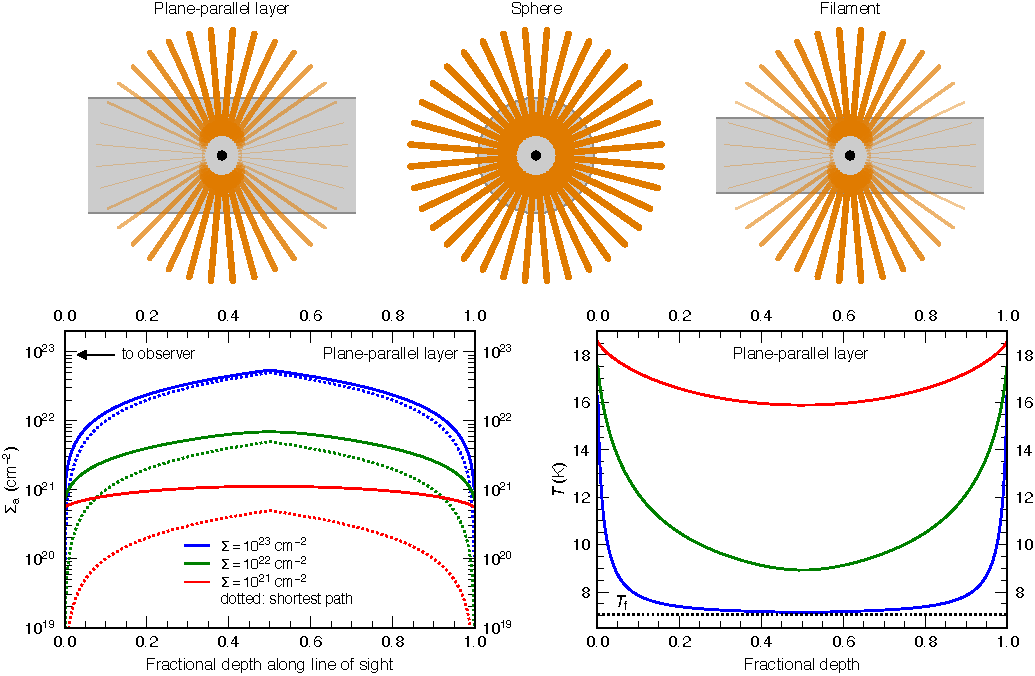
\includegraphics[width=0.93\linewidth]{fig_geometry.pdf}
\caption{\emph{Upper panels}: the radiation that heats a parcel of dust, marked by the black point, arrives from every direction
having crossed columns of very different length. The arrows are drawn thicker where less material has been crossed. In a layer
almost everything arrives along the normal; at the center of a sphere no direction is favored; a filament is intermediate, short
across and long along its axis. \emph{Lower left}: the effective attenuating column $\Sigma_{\rm a}$ of Eq.~(\ref{eq:seff}) against
the fractional depth along a line of sight through a layer, for total surface densities $\Sigma$ of $10^{21}$, $10^{22}$ and
$10^{23}$\,cm$^{-2}$. The dotted curves are the column along the shortest path, to the nearer surface of the layer. \emph{Lower
right}: the dust temperature that follows from $\Sigma_{\rm a}$ through Eq.~(\ref{eq:law}). The dotted line marks the floor
temperature $T_{\rm f}$.}
\label{fig:geometry}
\end{figure*}

The upper panels of Fig.~\ref{fig:geometry} illustrate this for the three shapes used to describe clouds. The arrows are thicker
where the radiation has crossed less material, so they show which directions deliver the energy. Deep inside a layer, the radiation
arrives almost entirely along the normal. A direction inclined by an angle $i$ crosses $1/\cos i$ times more material, and grazing
directions deliver nothing. At the center of a sphere, every direction crosses the same column, and no direction is favored. A
filament combines the two cases. Across the filament the path is short, and along its axis it is long. A filament therefore
resembles a sphere in its cross-section and a layer along its axis.

We do not want to carry an integral over directions into every pixel. We therefore replace the angular distribution by the single
column that gives the same mean intensity. We call it the effective attenuating column $\Sigma_{\rm a}$ and define it by
\begin{equation}
e^{-\kappa\,\Sigma_{\rm a}} \;=\; \left\langle e^{-\kappa\,\Sigma_{\rm a}(\hat n)}\right\rangle_{4\pi} .
\label{eq:seff}
\end{equation}
The column $\Sigma_{\rm a}$ is larger than the column along the shortest path, because the oblique directions deliver less
radiation than the shortest path does. The dust temperature depends on $\Sigma_{\rm a}$. Figure~\ref{fig:angular} in
Appendix~\ref{app:shape} shows how the average of Eq.~(\ref{eq:seff}) is formed at the mid-plane of a layer, and how $\Sigma_{\rm
a}$ grows with the total surface density of the line of sight.

We make two assumptions here. First, the opacity at the heating wavelengths is taken to be gray, with $A_{\rm V} =
\Sigma/(0.94\times10^{21}\,{\rm cm}^{-2})$ \citep{Bohlin+1978} and the optical depth $\tau = A_{\rm V}/1.086$. In reality, the
opacity varies across the ultraviolet and optical, so Eq.~(\ref{eq:seff}) is an average over wavelength as well as over direction.
Second, the radiation field outside the cloud is isotropic, as in the models of Sect.~\ref{sec:models}.

\subsection{The models}
\label{sec:models}

The relation between $\Sigma_{\rm a}$ and $T$ is not a free choice. It follows from radiative transfer, once the dust properties
and the radiation field are fixed. We computed a grid of models with \emph{radmc-3d} \citep{Dullemond+2012}. Each model is a
Bonnor--Ebert sphere \citep{Ebert1955, Bonnor1956} embedded in a uniform spherical cloud. It is heated from outside by the
interstellar radiation field, of strength $G_0 = 10$ in the units of \citet{Habing1968}. The field is that of \citet{Black1994},
with $G_0 = 0.98$, plus a hot blackbody component that is scaled to reach the required $G_0$. The models also include the cosmic
microwave background.
The dust opacity is that of \citet{Ossenkopf+Henning1994}, scaled to the power law $\kappa_\nu = \kappa_0(\nu/\nu_0)^2$ with
$\kappa_0 = 10.0$\,cm$^2$\,g$^{-1}$ (of dust) at $\nu_0 = 1000$\,GHz. The dust-to-gas mass ratio is $10^{-2}$ and $\muH = 2.8$.
The main grid contains 2089 models. They span the surface density of the embedding cloud, the size of the core, and its
central-to-edge density ratio (Appendix~\ref{sec:grid}). Three models reach the highest surface densities and are optically thick
in the far infrared. The correction assumes optically thin emission, so we leave these three models out. The relation is fitted to
the other 2086 models and to the models of filaments described below.

Filaments are not spheres, so we also computed models of filaments. Each one is a cylinder with the density profile $\rho(R) =
\rho_{\rm c}\,[1 + (R/R_{\rm f})^2]^{-p/2}$, truncated at the radius $R_{\rm out} = 0.5$\,pc. The flat radius $R_{\rm f}$ is
set by the half-maximum width $H$ of the surface density profile. The cylinders are isolated: no cloud surrounds them. They are
computed with the same dust and the same radiation field as the spheres, on an axisymmetric grid with a length of 7.2\,pc. We use
only their middle part, where the temperature depends on $R$ alone. We computed eight cylinders. Six of them have $p = 1.75$, $H =
40{\arcsec}$, and surface densities on the axis of $3{\times}10^{21}$, $10^{22}$, $3{\times}10^{22}$, $5{\times}10^{22}$,
$10^{23}$ and $2{\times}10^{23}$\,cm$^{-2}$. The other two have $3{\times}10^{22}$\,cm$^{-2}$ on the axis, with $p = 2$ or with
$H = 80{\arcsec}$. The cylinder with $2{\times}10^{23}$\,cm$^{-2}$ has an optical depth of 0.84 at 100{\um} through its axis, like
the three spheres that we left out, so we leave it out as well. For each cylinder, $\Sigma_{\rm a}$ is computed from
Eq.~(\ref{eq:seff}) for an infinite cylinder with the same profile. The spheres and the cylinders are given equal total weights in
the fit. The models of cylinders must be computed on a grid that covers both sides of their equatorial plane. With the mirror
symmetry of \emph{radmc-3d}, their temperatures come out too low by up to 1\,K (Appendix~\ref{app:rtmodels}).

The density structure of every model is known. The attenuating column of a shell can therefore be computed along any direction by
integrating the density along that ray. Equation~(\ref{eq:seff}) is then evaluated by summing over directions. Each shell is
weighted by its mass. Near the centers of the densest cores, few photon packets of the Monte Carlo calculation arrive, and the
temperatures of the innermost cells scatter widely. We reject a shell among the ten innermost ones if its temperature differs by
more than 10\% from the median of its five neighbors. We also reject every shell inside it. The rejected shells are 1.8\% of all
shells, and they contain a negligible fraction of the mass. The fit does not depend on this choice.

\subsection{The relation}
\label{sec:relation}

The 102\,464 shells of the 2086 spheres and the 315 radii of the seven cylinders follow a single relation
(Fig.~\ref{fig:shielding}). We fit it with the function
\begin{equation}
T(\Sigma_{\rm a}) = T_{\rm f} + (T_0 - T_{\rm f}) \left(1 + \frac{\Sigma_{\rm a}}{\Sigma_\star}\right)^{-\gamma},
\label{eq:law}
\end{equation}
where $T_{\rm f} = 7.0454$\,K, $T_0 = 22.8302$\,K, $\Sigma_\star = 2.7317\times10^{21}$\,cm$^{-2}$ and $\gamma = 1.6828$. The
mass-weighted scatter about the relation is 4.6\%. The two limits have simple meanings. $T_0$ is the temperature of dust that the
radiation reaches without attenuation. $T_{\rm f}$ is the temperature that dust approaches when the radiation cannot reach it at
all; the dust is then warmed only by the little radiation that penetrates and by the microwave background. The spheres and the
cylinders follow the same relation: on average, the spheres are 0.8\% warmer than the relation and the cylinders 0.3 to 0.9\%
colder. Leaving out any one cylinder changes the correction factor by at most 2\%. Above $\Sigma_{\rm a} = 10^{23}$\,cm$^{-2}$, the
models contain too little mass to constrain the relation.

\begin{figure}
\centering
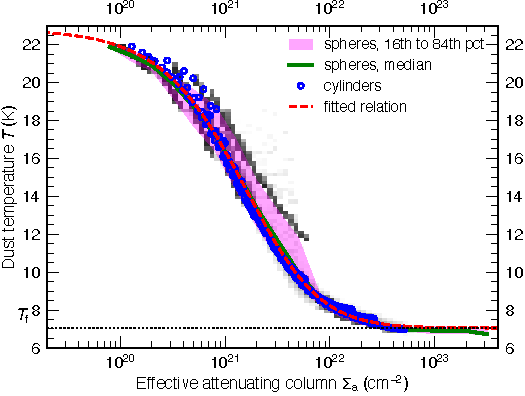
\includegraphics[width=0.98\columnwidth]{fig_shielding.pdf}
\caption{The dust temperature against the effective attenuating column $\Sigma_{\rm a}$ in the radiative transfer models. The gray
scale is the mass-weighted density of the 102\,464 shells of the 2086 spheres. The solid line and the band are their weighted
median and their 16th to 84th percentiles in bins of 0.2\,dex. The circles are the 315 radii of the seven cylinders. The dashed line
is the relation of Eq.~(\ref{eq:law}), fitted to the spheres and the cylinders with equal weights. The dotted line marks the
temperature $T_{\rm f}$ that fully shielded dust approaches.}
\label{fig:shielding}
\end{figure}

A single relation describes models that differ greatly from one another. This is the result that makes the method possible. The
size of a core and its concentration do not appear in Eq.~(\ref{eq:law}), and they do not need to. They affect the temperature only
by changing the amount of material between the dust and the radiation. The scatter about the relation, 4.6\%, measures how much
structures of different shapes differ at the same $\Sigma_{\rm a}$. It is physical, and it would not decrease with more models.

% =====================================================================

\section{The correction}
\label{sec:corr}

\begin{figure*}
\centering
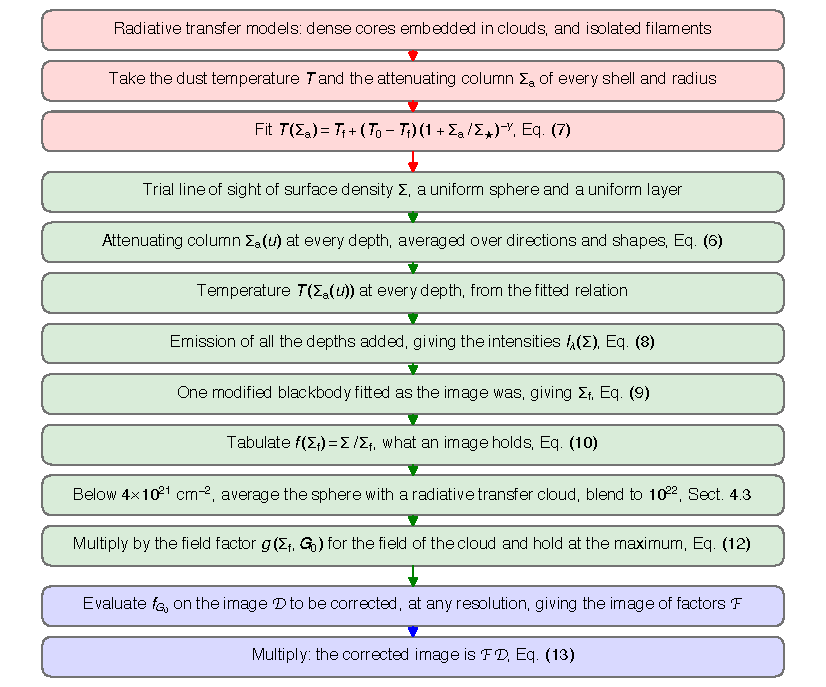
\includegraphics[width=0.76\textwidth]{fig_method.pdf}
\caption{The method step by step. The first group is the calibration, which is done once and yields the temperature relation of
Eq.~(\ref{eq:law}). The second is the calculation of Sect.~\ref{sec:factor}, repeated for every trial surface density, which
yields the table of the correction factor against the surface density that an observed image actually holds. Its last two steps
calibrate the low surface densities on a radiative transfer model of a diffuse cloud (Sect.~\ref{sec:diffuse}) and adapt the factor
to the radiation field of the cloud (Sect.~\ref{sec:g0corr}). The third group is
what is then done to an image, at any resolution.}
\label{fig:method}
\end{figure*}

\subsection{The calculation}
\label{sec:factor}

We now have everything we need. Apart from the calibration of diffuse material (Sect.~\ref{sec:diffuse}), nothing is left to
adjust. For a line of sight with the true surface density $\Sigma$, the factor is computed in five steps. (\emph{i}) We take a
structure of uniform density with the total surface density $\Sigma$ and compute $\Sigma_{\rm a}$ at each depth from
Eq.~(\ref{eq:seff}), once for a uniform sphere along its diameter and once for a uniform plane-parallel layer along its normal. The
two values are averaged at each depth, for the reason given in Sect.~\ref{sec:orient}. (\emph{ii}) The temperature at each depth
follows from Eq.~(\ref{eq:law}). (\emph{iii}) The emergent intensity is the sum of the emission of all layers,
\begin{equation}
   \Iim_\lambda(\Sigma) = \kappa_\lambda\,\eta_{\rm dg}\,\muH\,\mH\,\Sigma
   \int_0^1 B_\lambda \big(T(\Sigma_{\rm a}(u))\big)\,{\rm d}u ,
\label{eq:emission}
\end{equation}
where $u$ is the fraction of the total surface density that lies in front of a layer, $\kappa_\lambda$ is the dust opacity per unit
mass of dust, $\eta_{\rm dg} = 10^{-2}$ is the dust-to-gas mass ratio, and $\mH$ is the mass of a hydrogen atom. (\emph{iv}) We fit a single modified blackbody to these intensities, in the same wavebands and with the same weights as the
reconstruction. The fit gives a temperature $\Teff$ and the surface density that the reconstruction would report. It is
obtained from the reference waveband, which is the longest one, 500{\um}:
\begin{equation}
   \Sigma_{\rm f}(\Sigma) = \frac{\Iim_{\rm ref}(\Sigma)} {\kappa_{\rm ref}\,\eta_{\rm dg}\,\muH\,\mH\,B_{\rm ref}(\Teff)} ;
\label{eq:fitted}
\end{equation}
(\emph{v}) The correction factor is the ratio of the two surface densities. It is tabulated against $\Sigma_{\rm f}$, because an
observed image contains $\Sigma_{\rm f}$ and not $\Sigma$:
\begin{equation}
   f(\Sigma_{\rm f}) = {\Sigma}/{\Sigma_{\rm f}} .
\label{eq:factor}
\end{equation}
Figure~\ref{fig:method} shows the five steps together with the steps before and after them.

\begin{figure}
\centering
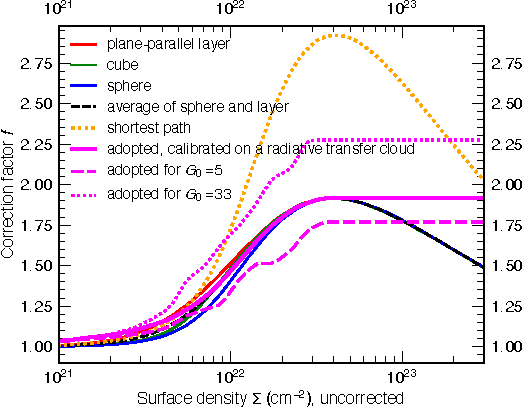
\includegraphics[width=0.98\columnwidth]{fig_relation.pdf}
\caption{The correction factor against the surface density of the uncorrected image, for a uniform plane-parallel layer, for a cube,
for a uniform sphere, and for the average of the sphere and the layer. The dotted curve uses the column along the shortest path
instead of the angular average (Appendix~\ref{app:shape}). The thick magenta curve is the adopted relation for $G_0 = 10$. Below
$10^{21.6}$\,cm$^{-2}$ it replaces the analytic layer by a radiative transfer model of a diffuse cloud (Sect.~\ref{sec:diffuse}), and
above its maximum it is held constant (Sect.~\ref{sec:factor}). The thin magenta curves are the adopted relation for $G_0 = 5$ and 33,
with the field factor of Eq.~(\ref{eq:factorg0}).}
\label{fig:relation}
\end{figure}

Figure~\ref{fig:relation} shows the result. For the analytic structures, the factor is unity below $10^{21}$\,cm$^{-2}$, where
nothing is attenuated. It rises steeply through the range of surface densities of most of a molecular cloud. It reaches its maximum,
1.92, near $3{\times}10^{22}$\,cm$^{-2}$ and then declines, to 1.47 at $3{\times}10^{23}$\,cm$^{-2}$. At such surface densities,
most of the material of a uniform body has reached the temperature floor, so its line of sight is again nearly isothermal. Real
dense structures are not uniform. A concentrated core has a cold center inside a warmer envelope, and its temperature still varies
along the line of sight. The radiative transfer models confirm this: the factor that they require stays at 2.0 to 2.4 up to
$10^{23}$\,cm$^{-2}$, where the models end. The decline of the analytic relation is therefore an artifact of the uniform bodies. We
hold the factor at its maximum above the surface density at which it is reached, so that it never decreases with the surface
density. The adopted relation differs from the analytic one in this respect and below $10^{22}$\,cm$^{-2}$, for the reason given in
Sect.~\ref{sec:diffuse}.

The lower left panel of Fig.~\ref{fig:geometry} shows the quantity that drives the calculation, the profile of $\Sigma_{\rm a}$ along a
line of sight. At $10^{21}$\,cm$^{-2}$ the profile is nearly flat. The line of sight is then nearly isothermal, and there is almost
nothing to correct. As the surface density rises, the profile steepens and approaches the dotted line of the shortest path. Once
the material is optically thick, the oblique directions deliver nothing, and only the normal direction matters.


\subsection{Why the shape hardly matters}
\label{sec:orient}

The calculation needs a shape, but an observed field does not provide one. Cores are embedded in filaments. Filaments are curved
and blended with their neighbors. Everything lies on a background that fluctuates on all scales. It is therefore important that the
result should not depend much on the assumed shape. It does not.

Figure~\ref{fig:relation} gives the factor for a uniform sphere, a uniform cube and a uniform plane-parallel layer of the same
observed surface density. The three agree to within 10\% everywhere. Outside the range from $10^{21.4}$ to
$10^{22.1}$\,cm$^{-2}$, they agree to within 4\%. Figure~\ref{fig:geometry} shows why. At low surface densities nothing is attenuated, and every shape gives $f = 1$. At
high surface densities the deepest material is optically thick in every direction, and the distribution of path lengths no longer
matters. The shape matters only in between, where the correction itself is modest. In short, where the geometry would matter, the
correction is small, and where the correction is large, the geometry does not matter. We adopt the average of the sphere and the
layer, and we take half of their difference, at most 5\%, as the uncertainty due to the geometry.

Appendix~\ref{app:shape} explains why the sphere and the layer are the two limits. It also explains why the angular average cannot
be replaced by the column along the shortest path.

One assumption remains: each structure is taken to have a uniform density. This assumption matters much less than it seems. For a
plane-parallel line of sight it does not matter at all. A parcel of dust is shielded by the column between the parcel and the
surface. This column does not depend on how the material within it is distributed. Putting half of the material into a dense clump
does not change the amount of material. The mass of a line of sight per unit column is also constant for any density profile,
because the column is the integral of the density. Let $\Sigma(s)$ be the column in front of a parcel at the depth $s$. The emission of
Eq.~(\ref{eq:emission}) integrated along the line of sight is then
\begin{equation}
   \int_0^L B_\lambda\big(T(\Sigma_{\rm a}(\Sigma(s)))\big)\,\rho(s)\,{\rm d}s
   = \int_0^{\Sigma} B_\lambda\big(T(\Sigma_{\rm a}(\Sigma^{\prime}))\big)\,{\rm d}\Sigma^{\prime} ,
\label{eq:invariance}
\end{equation}
and the density has disappeared. Two lines of sight with the same total surface density emit the same spectrum. It does not matter
whether their material is smooth or clumped, or whether a clump lies at the near side, in the middle, or at the far side.
Appendix~\ref{app:arrange} confirms this numerically for density profiles that differ by a factor of thirty. They reproduce the
smooth case to two parts in $10^{4}$.

Concentration and arrangement can therefore act only through the one thing that Eq.~(\ref{eq:invariance}) assumes: that the
radiation escapes along the line of sight and not across it. Their effect is modest. A sphere with a central-to-edge density ratio
of 10 needs a correction 2 to 4\% larger than a uniform sphere of the same central surface density. For a ratio of $10^3$, it needs
8 to 19\% more, and the difference grows with the surface density. A diffuse cloud with a denser structure embedded in it is a
different case. The correction for such a line of sight is between 13\% too small and 23\% too large, depending on the depth of the
structure in the diffuse cloud. Both effects are measured in Appendix~\ref{app:arrange}, and they enter the uncertainties of
Appendix~\ref{sec:limits}.

\subsection{Diffuse material}
\label{sec:diffuse}

The relation of Eq.~(\ref{eq:law}) was measured on spheres and cylinders. These are bounded structures. Most of the area of a
molecular cloud, however, is covered by extended diffuse material, which we call the diffuse cloud, or simply the cloud. It forms
the background on which the filaments and cores are seen. We therefore computed a radiative transfer model of such material
(Appendix~\ref{app:rtmodels}). It is a cube 2\,pc deep whose projection is the map of the cloud of our simulated sky, with surface
densities from $3\times10^{20}$ to $3\times10^{22}$\,cm$^{-2}$. In each column of the cube, one modified blackbody was fitted to
the emission at 160 to 500{\um}, and the result was compared with the true surface density.

The analytic layer, which enters the average of Sect.~\ref{sec:orient}, does not describe this cloud. The layer needs almost no
correction below $10^{21}$\,cm$^{-2}$, but the radiative transfer model of the cloud needs 5\% even at $5\times10^{20}$\,cm$^{-2}$,
and 15--25\% at a few $10^{21}$\,cm$^{-2}$. The reason is the surface of the cloud. Its outer layers are heated by the unattenuated
ultraviolet radiation from half the sky. They are up to 3\,K warmer than Eq.~(\ref{eq:law}) predicts, because that relation
describes the attenuation with a single gray opacity. The temperature therefore varies more along a line of sight through the cloud
than through the analytic layer, and the fit loses more.

We therefore replace the analytic layer by the radiative transfer model of the cloud at low surface densities. Below a fitted
surface density of $10^{21.6}$\,cm$^{-2}$, the factor is the average of the analytic sphere and of the factor measured on the
cloud. Between $10^{21.6}$ and $10^{22}$\,cm$^{-2}$, it changes smoothly into the analytic average of sphere and layer, which is
used above. The factor is thus 1.03 at $3\times10^{20}$\,cm$^{-2}$ and 1.12 at $3\times10^{21}$\,cm$^{-2}$, against 1.00 and 1.07
for the analytic average. It remains a function of the surface density alone. The bounded spheres and the extended cloud are the
two limits for diffuse material, as the sphere and the layer are for a single structure. Their average divides the uncertainty
between them. A uniform cloud around a core is corrected about 2\% too much (Sect.~\ref{sec:valgrid}). The radiative transfer
model of the cloud is corrected too little, by 6\% at $10^{21}$\,cm$^{-2}$ and by 14\% at $10^{22}$\,cm$^{-2}$, with a median of
11\% (Sect.~\ref{sec:sim}).

\subsection{The radiation field of a cloud}
\label{sec:g0corr}

The relation of Eq.~(\ref{eq:law}) and the factor $f$ are calibrated for $G_0 = 10$. Clouds are heated by very different fields. The
diffuse material of the regions listed in Appendix~\ref{app:fieldest} requires fields from below 1 to about 250. A stronger field
heats the dust at every attenuating column, and it changes the temperature contrast along the line of sight. The factor that a
line of sight requires therefore depends on the field (Appendix~\ref{sec:field}).

We measured this dependence on the grid of radiation fields of Appendix~\ref{sec:grid}, which repeats the models in nine fields from
$G_0 = 0.98$ to 483. For each field, we took the factor that each pixel of each model requires, and averaged its logarithm in bins of
0.1\,dex of the fitted surface density $\Sigma_{\rm f}$. The ratio of this average to the same average at $G_0 = 10$ is the field factor
$g(\Sigma_{\rm f}, G_0)$. Above $10^{22.6}$\,cm$^{-2}$, the grid contains too few pixels to determine it, and $g$ is held at its value
there. Between the fields of the grid, $\log g$ is interpolated linearly in $\log G_0$. The field factor is within 3\% of unity below
$10^{21.4}$\,cm$^{-2}$ in every field. At $10^{22}$\,cm$^{-2}$, it is 0.80 for $G_0 = 1$, 0.91 for $G_0 = 5$, 1.16 for $G_0 = 33$,
and 1.09 for $G_0 = 250$ (Appendix~\ref{app:field}).

The factor applied to a cloud in the field $G_0$ is then
\begin{equation}
f_{G_0}(\Sigma_{\rm f}) = \max_{\Sigma^{\prime} \le \Sigma_{\rm f}} \Big[ f(\Sigma^{\prime})\,g(\Sigma^{\prime}, G_0) \Big] ,
\label{eq:factorg0}
\end{equation}
which also holds the factor at its maximum (Sect.~\ref{sec:factor}). For $G_0 = 10$, $g = 1$. The field is a single number for a
cloud. It is the field that the models require to reproduce the observed temperatures, an effective field of the model dust, which
can differ from the physical field. It is estimated from the temperatures of the diffuse material of the whole map, with the procedure of
Appendix~\ref{app:fieldest}. It is not read from the temperature of each pixel, which is ambiguous (Appendix~\ref{app:tcorr}). The
correction therefore still depends on the surface density alone, and the field is an input of the calculation, like the wavebands.

\subsection{How it is applied}
\label{sec:apply}

An image is corrected by multiplying it by the image of the correction factors evaluated on the image itself,
\begin{equation}
\Sc(\theta) = \mathcal{F}(\theta)\,\Sim(\theta), \quad \mathcal{F}(\theta) \equiv f_{G_0}\big(\Sim(\theta)\big) ,
\label{eq:correction}
\end{equation}
where $f_{G_0}$ of Eq.~(\ref{eq:factorg0}) is evaluated pixel by pixel. Without an estimate of the field, $G_0 = 10$ is used.
This applies to every image of a reconstruction, at any resolution $\theta$, and to a conventional surface density map. The factor
was calibrated for the surface density that a single modified blackbody fit returns at the resolution of the longest waveband. An
image at a finer resolution is sharper than any such fit. Appendix~\ref{sec:deficit} shows that its fractional deficit is
nevertheless the same, and the tests of Sect.~\ref{sec:valid} confirm it. There is an alternative. The factor can be evaluated on
a coarser image of the reconstruction, and the correction $[f - 1]\,\Sim$ of that image added to every finer image.
Equation~(\ref{eq:cumulative}) allows this, because the increments do not depend on the coarsest image. Section~\ref{sec:base}
compares the two ways. We adopt the first, which gives the sharper images and, on the radiative transfer models, the more accurate
masses. The correction must be applied only once. Our two implementations of the correction, in Fortran and in Python, mark their
output and refuse an input that has already been corrected. Both are distributed as part of \emph{getsf} on its home
page\footnote{\url{http://irfu.cea.fr/Pisp/alexander.menshchikov/}}.

\subsection{What the correction needs, and what it does not}
\label{sec:needs}

Nothing in Eqs.~(\ref{eq:seff}) to (\ref{eq:factor}) refers to the multi-resolution reconstruction. For a given field, the factor is a
function of one number: the surface density that a single modified blackbody fit returns at the resolution of the longest
waveband. This number can
be obtained from the observed images alone. The base image of \emph{hires} is exactly this fit. We verified this on the grid: a
modified blackbody fitted to the same wavebands with the same weights reproduces the base image of \emph{hires} to better than 1\%
for every model. The correction therefore applies to a conventional surface density map, made in the usual way from the
\emph{Herschel} intensities convolved to a common beam. Equation~(\ref{eq:correction}) then reduces to multiplying that map by
$f$.

What the reconstruction adds, and what no correction can replace, are the increments. They contain the information on scales finer
than the beam of the longest waveband. Without them, there is nothing to correct at $13.5{\arcsec}$, and the corrected map is a map
at $36.3{\arcsec}$.

The order of the operations matters when an image is decomposed into components. A parcel is shielded by the whole column along its
line of sight. The factor must therefore be evaluated on the total surface density, not on a component of it. The image must be
corrected first, and the background of a structure subtracted afterwards. If the background is subtracted first, the factor is
evaluated at a surface density that the material does not have, and the structure is corrected much too little. For the same
reason, the correction must never be applied to an image that is already corrected, or to a true surface density.

One condition applies when the correction is used outside \emph{hires}. The table of $f$ is built for a particular set of wavebands
and a particular weighting of them, because $\Sigma_{\rm f}$ depends on both. The table must be rebuilt if a map was made from other
wavebands or with other weights. The table cannot be replaced by anything derived from the photometry itself, for the reason given
in Appendix~\ref{app:colors}. The signature of the temperature mixing is smaller than the calibration uncertainties, so the
correction must come from models.

Two more properties follow from the construction. First, the correction is insensitive to noise, because it evaluates a smooth
function of an image and fits nothing. We added Gaussian noise of 1.5, 0.50, 0.30 and 0.15\,MJy\,sr$^{-1}$ at 160, 250, 350 and
500{\um} to the models. The total corrected surface density changed by less than 0.5\%. Second, the correction does not amplify
the calibration errors of the wavebands much. The amplification by 7 to 9 found in Appendix~\ref{app:colors} does not apply here,
because the deficit is not derived from the colors. A calibration error changes the fitted surface density $\Sigma_{\rm f}$, and the
corrected surface density $f(\Sigma_{\rm f})\,\Sigma_{\rm f}$ follows. We computed the effect of an error of 10\% in each waveband for
uniform lines of sight of $3{\times}10^{21}$ to $10^{23}$\,cm$^{-2}$. An error at 500{\um}, the reference waveband, changes the
uncorrected surface density by 16 to 18\% and the corrected one by 16 to 23\%. An error at 160, 250 or 350{\um} changes the
fitted temperature by up to 0.4\,K. It changes the uncorrected surface density by 1 to 12\% and the corrected one by 1 to 11\%. An
error of 10\% in all wavebands at once changes the uncorrected surface density by 10\% and the corrected one by 9 to 13\%. Where $f$
rises steeply with $\Sigma_{\rm f}$, between $10^{22}$ and $3{\times}10^{22}$\,cm$^{-2}$, the correction enlarges the error of the
uncorrected image by up to 1.4 times. Where $f$ declines, at the highest surface densities, it reduces the error slightly.

% =====================================================================


\section{Validation}
\label{sec:valid}

A correction can be tested only where the true surface density is known. We test it in three settings, all computed with
radiative transfer. The first is a grid of models of cores, each in its own uniform cloud. The second is a set of isolated
filaments. The third is a simulated sky, in which a cloud, filaments and cores overlap along the lines of sight. All of them are
computed for $G_0 = 10$, so $g = 1$ in Eq.~(\ref{eq:factorg0}). Holding the factor at its maximum changes it only above
$10^{22.6}$\,cm$^{-2}$. Within the surface densities of these models, the change is at most 2\%, and the results below are given
without it. The correction for other fields is tested in Appendix~\ref{sec:field}.

\subsection{On radiative transfer models of cores}
\label{sec:valgrid}

The relation of Eq.~(\ref{eq:law}) was fitted to the models of the main grid. To test the correction on models that were not used
in the fit, we computed a second grid of 1815 models. Their parameters lie between those of the main grid, and they have the same
radiation field $G_0 = 10$ (Appendix~\ref{sec:grid}). For each model, we convolved the emission to the beams of the four wavebands
and reconstructed it with \emph{hires}, as for an observation. We then corrected the image at $13.5{\arcsec}$ with the factor
evaluated on that image and, for comparison, with the factor evaluated on the image at $36.3{\arcsec}$. We compared the corrected
images with the true surface density of the model at the same resolution in three ways. Table~\ref{tab:valgrid} gives the results.

The first measure is the accuracy ratio of the total surface density within the footprint of the model, that is, the total in the
corrected image divided by the same total in the true image.
The footprint is the area where the model stands above its surroundings in the true image at $13.5{\arcsec}$. This measure shows
whether the correction restores the right amount of material. The second measure is the mass $M$ of the core. It is the same
total with the background subtracted, divided by the same quantity in the true image. The background is the median surface density
in a ring $15{\arcsec}$ wide just outside the footprint. The mass is measured for 1750 of the models. For the other 65 models, the ring
contains fewer than 20 valid pixels, because the footprint reaches the edge of the image, or the true mass within the footprint is not
positive, because the core barely stands above its cloud. The third measure is the radial profile of the relative residual. The
residual is the corrected minus the true surface density, divided by the true surface density, as a function of the distance from
the center of the core. Each measure is computed for every model. Table~\ref{tab:valgrid} gives the median over the models and the
16th and 84th percentiles, which enclose 68\% of the models (one standard deviation from the mean of a Gaussian).

\begin{table}
\caption{Validation on 1815 radiative transfer models that were not used to fit the relation of Eq.~(\ref{eq:law}). Total: the
accuracy ratio of the surface density summed over the footprint of the model. Core mass: the accuracy ratio of the same sum less the
background, for the 1750 models in which the mass can be measured. Center and $21{\arcsec}$: the relative residual of the surface
density at 3 and $21{\arcsec}$ from the center of the core. The rows give the image before the correction and after it, with the
factor evaluated on the image at $36.3{\arcsec}$ or at $13.5{\arcsec}$. The first two columns give the median over the models, with 
the 16th and 84th percentiles in parentheses; the last two give medians.}
\label{tab:valgrid}
\centering
\begin{tabular}{lcccc}
\hline\hline
\noalign{\smallskip}
\!\!\! Image & \!\!\!\! Total & \!\!\!\! Core mass & \!\!\!\!\! Center & $21{\arcsec}$\!\!\\
\noalign{\smallskip}
\hline
\noalign{\smallskip}
\!\!\! uncorr.              & \!\!\!\!\! 0.78 (0.56--0.93) & \!\!\!\!\! 0.63 (0.46--0.86) & \!\!\!\!\!\!\! $-0.44$ & \!\!\!\!\!\!\! $-0.21$\!\!\\
\!\!\! $f$ at $36.3{\arcsec}$ & \!\!\!\!\! 0.99 (0.92--1.02) & \!\!\!\!\! 0.94 (0.71--1.09) & \!\!\!\!\!\!\! $-0.15$ & \!\!\!\!\!\!\! $+0.01$\!\!\\
\!\!\! $f$ at $13.5{\arcsec}$ & \!\!\!\!\! 0.99 (0.93--1.02) & \!\!\!\!\! 0.98 (0.76--1.12) & \!\!\!\!\!\!\! $-0.12$ & \!\!\!\!\!\!\! $+0.02$\!\!\\
\noalign{\smallskip}
\hline
\end{tabular}
\end{table}

\begin{figure*}
\centering
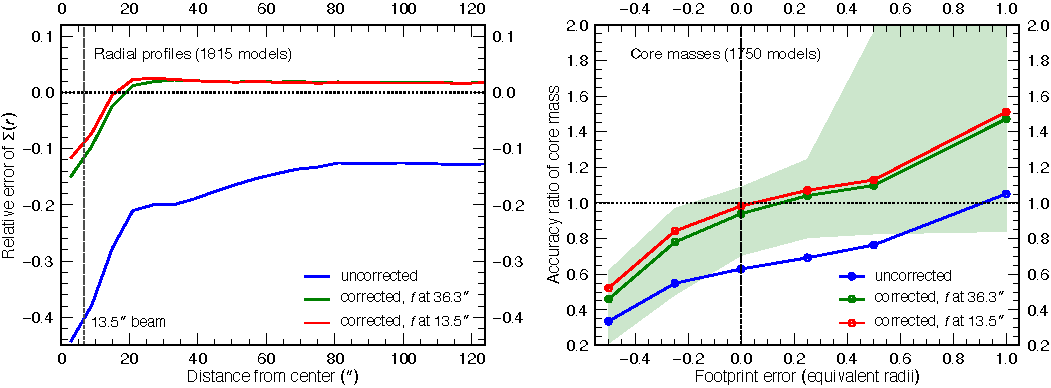
\includegraphics[width=0.98\textwidth]{fig_grid_validation.pdf}
\caption{The correction tested on 1815 radiative transfer models that were not used to fit the relation of
Eq.~(\ref{eq:law}). \emph{Left}: the relative residual of the surface density, the reconstructed minus the true value divided by
the true value, against the distance from the center of the core, as the median over the models. The dashed line marks half the
beam of $13.5{\arcsec}$. \emph{Right}: the accuracy ratio of the core mass, for the 1750 models in which it can be measured, when
the footprint within which it is
measured is too small (negative abscissa) or too large (positive abscissa) by the given fraction of its equivalent radius. The
background is always taken in a ring just outside the footprint used. The lines are medians over the models, and the band marks
the 16th to 84th percentiles for the factor evaluated at $36.3{\arcsec}$.}
\label{fig:valgrid}
\end{figure*}

Without the correction, the reconstruction contains 78\% of the true surface density and 63\% of the core mass. The deficit is
largest at the center of the core, where it reaches 44\%. The correction restores the total to 99\% and the core mass to 98\% in the
median. Beyond $15{\arcsec}$ from the center, the corrected surface density is about 2\% too high (Fig.~\ref{fig:valgrid}, left).
This is the uniform cloud around the core, which the calibration of Sect.~\ref{sec:diffuse} corrects slightly too much. A deficit of
12\% remains at the center of the core, at $3{\arcsec}$. No correction that depends on the surface density alone can remove it. The
center of a core is colder than the center of a uniform structure with the same surface density, and the surface density does not
reveal this. The factor evaluated at $36.3{\arcsec}$ gives almost the same totals but a larger deficit at the center 
(Sect.~\ref{sec:base}).

The spread over the models is larger than these medians. For one core in six, the corrected mass is more than 24\% too low. For
another one in six, it is more than 12\% too high. A correction that depends on the surface density alone cannot remove this
spread. Models with the same surface density can differ in how their temperature varies along the line of sight.

In a real image, the footprint of a core is not known. It must be estimated, together with the background beneath the core. The
right panel of Fig.~\ref{fig:valgrid} shows how an error in the footprint changes the measured mass. A footprint that is too small
by a quarter of its radius lowers the median corrected mass from 0.98 to 0.84 of the true mass. A footprint that is too small by
half its radius lowers it to 0.52, because part of the core is then counted as background. A footprint that is too large by a
quarter or a half of its radius raises the median mass to 1.07 or 1.13, and the spread over the models widens sharply. These errors
are lower limits. The models lie in a cloud of uniform density, whose surface density declines smoothly with radius. A real core is
surrounded by filaments and other cores. They enter the background ring in ways that no model reproduces.

\subsection{On radiative transfer models of filaments}
\label{sec:cyl}

The seven cylinders of Sect.~\ref{sec:models} were also imaged and reconstructed like an observation. They are isolated, so their
profiles are not confused by any background. Figure~\ref{fig:cylinders} and Table~\ref{tab:cyl} give the results, measured on
the median profile over the middle part of each cylinder. The true profile is convolved to the beam of $13.5{\arcsec}$.

\begin{table*}
\caption{The isolated radiative transfer cylinders at $13.5{\arcsec}$. $\Sigma_0$: the true surface density on the axis.
Crest: the accuracy ratio of the surface density on the axis, before and after the correction. $\Lambda$: the accuracy ratio of
the linear density within $\pm300{\arcsec}$, before and after. $H$: the half-maximum width of the true, the uncorrected and the corrected
profile. $\alpha$: the slope of $\log\Sigma$ against $\log r$ between 20 and $120{\arcsec}$ from the crest, for the same three
profiles.}
\label{tab:cyl}
\centering
\begin{tabular}{lcccc}
\hline\hline
\noalign{\smallskip}
$\Sigma_0$ (cm$^{-2}$) & Crest & $\Lambda$ & $H$ (${\arcsec}$) & $\alpha$ \\
\noalign{\smallskip}
\hline
\noalign{\smallskip}
$3{\times}10^{21}$                  & 0.86 $\rightarrow$ 0.93 & 0.96 $\rightarrow$ 1.01 & \!48\, \,\,\,58\,\, 55  & 0.89\,\, 0.88\,\, 0.90 \\
$1{\times}10^{22}$                  & 0.66 $\rightarrow$ 0.83 & 0.87 $\rightarrow$ 0.97 & \!48\, \,\,\,71\,\, 61  & 0.89\,\, 0.81\,\, 0.87 \\
$3{\times}10^{22}$                  & 0.50 $\rightarrow$ 0.81 & 0.75 $\rightarrow$ 0.95 & \!48\, \,\,\,79\,\, 59  & 0.89\,\, 0.70\,\, 0.85 \\
$5{\times}10^{22}$                  & 0.46 $\rightarrow$ 0.83 & 0.68 $\rightarrow$ 0.95 & \!48\, \,\,\,75\,\, 59  & 0.89\,\, 0.67\,\, 0.88 \\
$1{\times}10^{23}$                  & 0.42 $\rightarrow$ 0.80 & 0.60 $\rightarrow$ 0.94 & \!48\, \,\,\,68\,\, 62  & 0.89\,\, 0.70\,\, 0.90 \\
$3{\times}10^{22}$, $p=2$           & 0.50 $\rightarrow$ 0.81 & 0.73 $\rightarrow$ 0.94 & \!47\, \,\,\,72\,\, 56  & 1.07\,\, 0.86\,\, 1.02 \\
$3{\times}10^{22}$, $H=80{\arcsec}$ & 0.53 $\rightarrow$ 0.89 & 0.71 $\rightarrow$ 0.95 &   85\,      122\,\, 91  & 0.80\,\, 0.59\,\, 0.76 \\
\noalign{\smallskip}
\hline
\end{tabular}
\end{table*}

\begin{figure*}
\centering
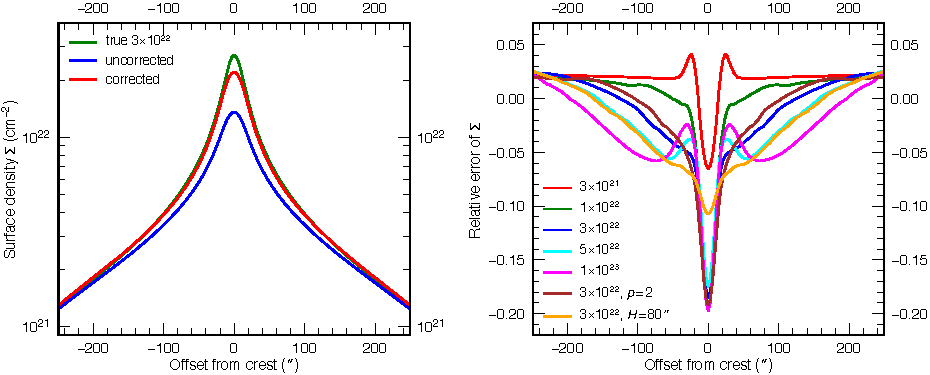
\includegraphics[width=0.95\textwidth]{fig_cylinders.pdf}
\caption{The isolated radiative transfer cylinders reconstructed by \emph{hires} at $13.5{\arcsec}$ and corrected. \emph{Left}: the
profile across the cylinder with $3{\times}10^{22}$\,cm$^{-2}$ on its axis, true (convolved to the beam), uncorrected and corrected.
\emph{Right}: relative error of the corrected surface density across all seven cylinders, labeled by their surface density on the 
axis. Each profile is the median over the middle part of the cylinder.}
\label{fig:cylinders}
\end{figure*}

Without the correction, the crests of the filaments are 14 to 58\% too low. The deficit grows with the surface density on the axis.
The linear densities are 4 to 40\% too low. The profiles are too wide and too shallow, because the crest is suppressed much more than
the wings. After the correction, the linear densities are within 6\% of the truth, and the slopes of the profiles are within 0.05
of the true ones. The crests remain 7 to 20\% too low. This is the same limit as at the centers of the cores: the axis of a filament
is colder than the middle of a uniform structure with the same surface density. For the same reason, the corrected widths $H$ are
still 15 to 30\% too large for the filaments of $40{\arcsec}$. For the filament of $80{\arcsec}$, which is well resolved, the width
is 7\% too large. Beyond about $20{\arcsec}$ from the crest, the corrected profiles are within 7\% of the truth.

\subsection{On a simulated sky}
\label{sec:sim}

The models of Sects.~\ref{sec:valgrid} and \ref{sec:cyl} each contain a single structure. An observed field does not. We therefore
built a simulated sky in which every component comes from radiative transfer, so that its emission and its surface density are
consistent. It contains a cloud, seven filaments and 96 cores, in a field of $1793 \times 1793$ pixels of $3{\arcsec}$
(Appendix~\ref{app:rtmodels}).

The cloud is the radiative transfer cube of Sect.~\ref{sec:diffuse}. Its surface density map has scale-free fluctuations and rises
toward the center of the field as a power law. Its median is $5\times10^{21}$\,cm$^{-2}$, and it reaches 2 to $3\times10^{22}$\,cm$^{-2}$
in the center. The seven filaments are the cylinders of Sect.~\ref{sec:cyl}. In the sky, each filament is embedded in the cloud:
it was computed again inside an envelope that shields it as the cloud around it does, and the envelope varies along the
filament as the cloud does. The emission of the envelope itself is then subtracted, so that only the filament is added to the
cloud. The filaments lie in the middle of the cloud, which is assumed to extend far in front of and behind them. The cores are the
radiative transfer models of the grid, each embedded in a cloud whose surface density matches its surroundings in the sky. The
intensities were convolved to the beams of the wavebands and reconstructed by \emph{hires}, as for an observation.

\begin{figure*}
\centering
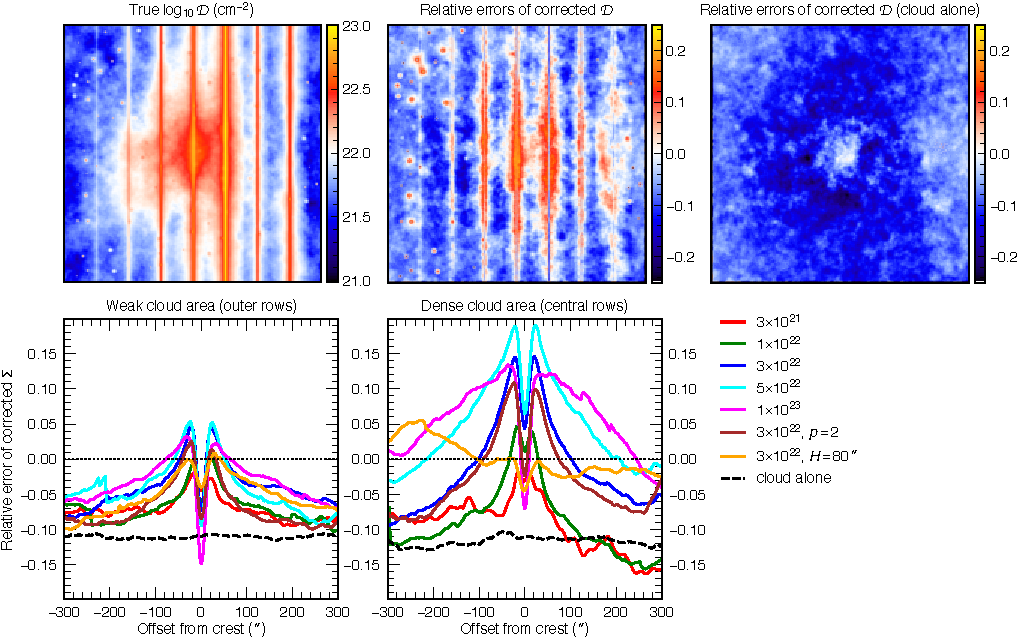
\includegraphics[width=\textwidth]{fig_simsky6.pdf}
\caption{The simulated sky, built from radiative transfer models of a cloud, seven filaments and 96 cores. \emph{Upper left}: the
true surface density at $13.5{\arcsec}$. \emph{Upper middle}: the relative error of the corrected surface density, (corrected $-$
true) / true. \emph{Upper right}: the same for a sky that contains the cloud alone. \emph{Lower panels}: the relative error
across each filament, as the median over the outer rows of the field, where the cloud is weak, and over its central rows, where
the cloud is dense. The filaments are labeled by their surface density on the axis. The cores are masked in the profiles. The
dashed curve is the cloud alone at the same positions.}
\label{fig:simsky6}
\end{figure*}

Figure~\ref{fig:simsky6} shows the result. We describe it component by component.

The cloud alone, in a sky without filaments and cores, is corrected to 0.89 of the truth in the median. The deficit is 6\% at
$10^{21}$\,cm$^{-2}$ and grows to 14\% at $10^{22}$\,cm$^{-2}$. Before the correction, the reconstruction contains 0.76 of the
truth. The fractional deficit is the same at $13.5{\arcsec}$ and at $36.3{\arcsec}$, within 0.5\%, which confirms the property
found in Appendix~\ref{sec:deficit}. The remaining deficit of the cloud is the price of the average of Sect.~\ref{sec:diffuse}, which
gives half the weight to the sphere.

In the outer parts of the field, the cloud is a few $10^{21}$\,cm$^{-2}$. There the crests of the filaments are corrected to
within 4 to 15\%, and their flanks to within 5\%. Their outer wings are corrected too little, by 6 to 10\%, as much as the
cloud around them.
In the center of the field, the cloud reaches 2 to $3\times10^{22}$\,cm$^{-2}$. There the flanks of the dense filaments are corrected
too much, by 10 to 19\%, while the cloud alone at the same positions is corrected too little. Both effects come from the
superposition of two structures, which a correction based on the surface density alone treats as one. They have the signs predicted
in Appendix~\ref{app:arrange}: a structure in a weak cloud is under-corrected, and a structure in a dense cloud is
over-corrected. The central cloud of the simulated sky is two to three times denser than the background of the filaments in Aquila,
which \emph{getsf} finds to be 6 to $10\times10^{21}$\,cm$^{-2}$ at most. In a field like Aquila, the over-correction of the flanks should
therefore be about 10\%.

Over the whole field, with the cores masked, the corrected surface density is 0.96 of the truth.

\subsection{Where the correction fails, and the resolution of the factor}
\label{sec:fails}
\label{sec:base}

Two kinds of structure are not corrected well by any correction that depends on the surface density alone. The centers of
concentrated structures, the centers of cores and the crests of filaments, remain 7 to 20\% too low. Cores narrower than two beams
keep a deficit of up to 40\% at their centers, surrounded by an over-corrected ring, because the beam spreads their cold centers over
an area of lower surface density. Superposed structures of very different temperatures are corrected too little or too much, by 10
to 20\% (Sect.~\ref{sec:sim}). Corrections that also read the fitted temperature do not help (Appendix~\ref{app:tcorr}).

The factor can be evaluated at any resolution. Evaluated on the image at $13.5{\arcsec}$, it gives core masses 5\% higher than
evaluated at $36.3{\arcsec}$, closer to the truth, and a smaller deficit at the centers (Table~\ref{tab:valgrid}). On the cloud of the
simulated sky, the two agree to 0.5\%. We therefore evaluate the factor on the image that is corrected. A factor evaluated at
$36.3{\arcsec}$ remains a conservative alternative.

% =====================================================================

\section{Application to the Aquila cloud}
\label{sec:aquila}

We applied the correction to a $31\arcmin \times 31\arcmin$ field of the Aquila cloud, centered at \draftnote{RA, Dec (J2000)}.
The field was observed with \emph{Herschel} \citep{Andre+2010, Konyves+2015}. The reconstruction uses the images at 160, 250, 350
and 500{\um}. We adopt a distance of 260\,pc. The field contains 375\,769 pixels of $3{\arcsec}$. The factor is evaluated on the
reconstruction at $13.5{\arcsec}$ and applied to it. Every pixel is corrected, including those toward protostars
(Appendix~\ref{sec:notdo}).

The radiation field of the cloud was estimated with the procedure of Appendix~\ref{app:fieldest}, from the diffuse material of the
whole Aquila map, which contains 29 million pixels. The field is $G_0 \approx 33$, with 25 and 41 for the 16th and 84th percentiles
of the temperature. The cloud is therefore heated by a field about three times stronger than the field of the calibration, and the
correction uses $G_0 = 33$ in Eq.~(\ref{eq:factorg0}).

The median correction factor over the field is 1.68. The factor is below 1.20, 1.54, 1.91 and 2.28 for 1, 25, 75 and 99\% of the
pixels, and it reaches its maximum, 2.28, above $3{\times}10^{22}$\,cm$^{-2}$. The correction is therefore significant everywhere in
the field. The total surface density of the field increases by a factor of 1.89. With the calibration field $G_0 = 10$, the median
factor would be about 1.45 and the total would increase by a factor of about 1.62.

The distribution of surface densities changes more than the median factor suggests, because the factor rises with the surface
density. The median surface density of the field increases from $9.7{\times}10^{21}$ to $1.6{\times}10^{22}$\,cm$^{-2}$, and its
99th percentile from $5.6{\times}10^{22}$ to $1.3{\times}10^{23}$\,cm$^{-2}$. The number of pixels above $10^{22}$\,cm$^{-2}$
increases from 178\,641 to 318\,215. Above $3{\times}10^{22}$\,cm$^{-2}$ it increases from 17\,041 to 85\,343, and above
$10^{23}$\,cm$^{-2}$ from 666 to 7049, a factor of 10.6. A much larger part of the cloud therefore exceeds any given threshold after
the correction. This matters for any criterion based on a surface density threshold, such as a threshold for star formation.

The corrected surface density implies a lower dust temperature. We define it as the temperature at which the corrected surface
density gives the same intensity at 500{\um} as the uncorrected surface density with the fitted temperature. Its median over the
field is 12.2\,K, against 15.0\,K for the fitted temperature. It is below 9.3 and 18.5\,K for 1 and 99\% of the pixels.

\begin{figure*}
\centering
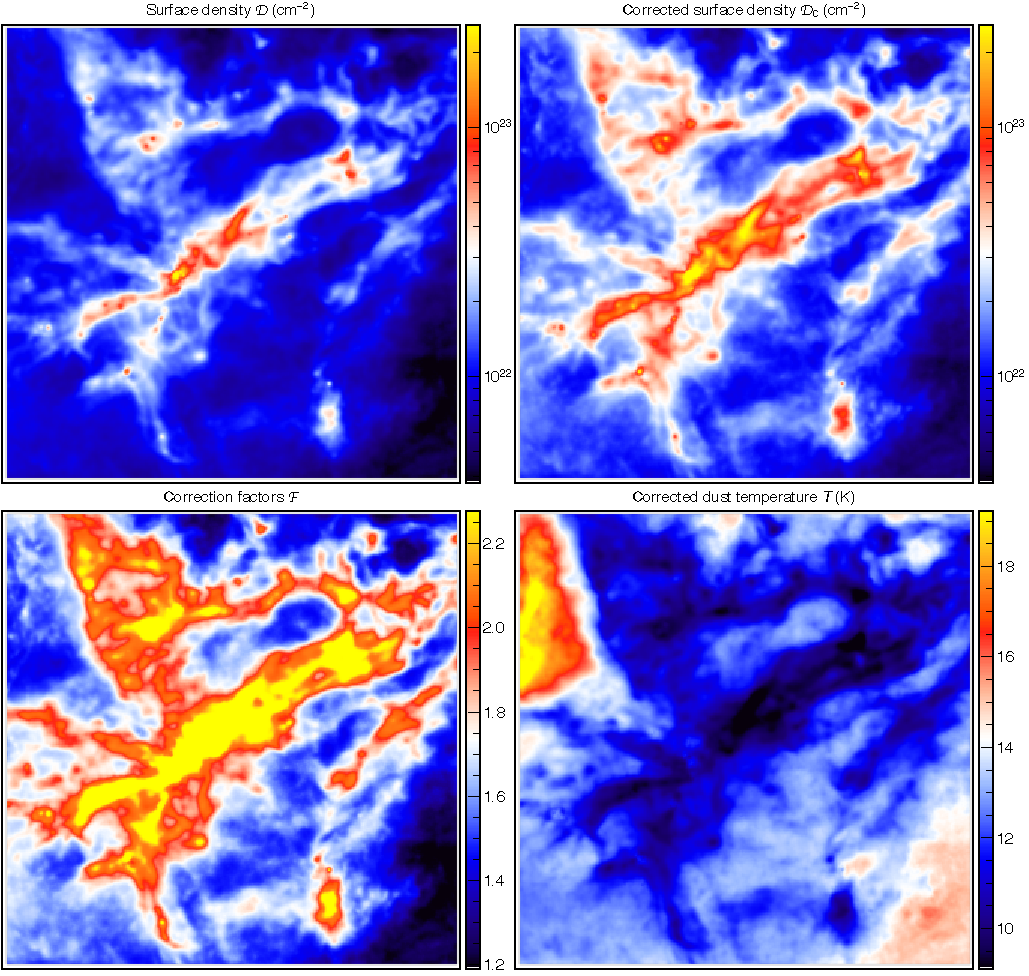
\includegraphics[width=\textwidth]{fig_aquila.pdf}
\caption{The Aquila field at $13.5{\arcsec}$, corrected for the field $G_0 = 33$. \emph{Upper panels}: the surface density before
and after the correction, on a common logarithmic scale. \emph{Lower panels}: the image of the correction factors $\mathcal{F}$ and
the corrected dust temperature (Sect.~\ref{sec:aquila}). The factor is smallest in the diffuse material and largest along the crests
of the filaments and at the cores.}
\label{fig:aquila}
\end{figure*}

Figure~\ref{fig:aquila} shows the field before and after the correction, together with $\mathcal{F}$ and the corrected dust
temperature. The correction is not a uniform rescaling. The factor is smallest in the diffuse material between the structures and
largest along the crests of the filaments and at the cores. The correction therefore raises the contrast of the image as well as its
overall level. Because the factor never decreases with the surface density, the densest crests and cores receive the largest
correction, and the corrected temperature shows no artificial dips toward them. The field is not uniform across the cloud. The
warm corner at the upper left of the temperature map is heated more strongly than the rest of the field, and there the single
field of the cloud underestimates the true one. Appendix~\ref{sec:field} discusses the uncertainty due to the radiation field.

\section{Conclusions}
\label{sec:conclusions}

Surface density images of molecular clouds are derived by fitting one modified blackbody to each pixel. These images are
systematically too low wherever the dust temperature varies along the line of sight. The deficit exceeds a factor of two in the
densest material.

The deficit cannot be measured from the observed colors. Its signature in the spectrum is 1 to 6\% of the intensities, while the
deficit itself is 9 to 38\%. A method that derived one from the other would amplify the photometric errors 7 to 9 times. The correction must therefore come from radiative transfer.

Radiative transfer provides a single relation between the dust temperature and the effective column $\Sigma_{\rm a}$ that shields
the dust. It describes 2086 models of embedded Bonnor--Ebert spheres and seven models of filaments, with a scatter of 4.6\%.
Because $\Sigma_{\rm a}$ is an average over all directions of the incoming radiation, a sphere, a cube and a plane-parallel layer of the
same surface density need factors within 10\% of each other. The relation gives the correction factor $f$ as an explicit function of
the observed surface density. At low surface densities, the factor is calibrated on a radiative transfer model of an extended
cloud, whose warm surface layers the relation does not describe.

The correction applies to a conventional surface density map at the resolution of the longest waveband and
to every image of a multi-resolution reconstruction. In a reconstruction, the deficit is the same fraction of the surface density at
every resolution. We evaluate the factor on the finest image, which gives the sharpest corrected images and the most accurate masses.

We tested the correction on three kinds of radiative transfer models. On 1815 models of cores that were not used in the
calibration, it raises the median core mass from 0.63 to 0.98 of the true mass and the total surface density from 0.78 to 0.99. On
seven isolated filaments, it restores the linear densities to 0.94--1.01 of the truth and the slopes of the profiles to within 0.05.
On a simulated sky of cloud, filaments and cores, all computed with radiative transfer, it restores the total surface density to
0.96. The centers of cores and the crests of filaments remain 7 to 20\% too low, because they are colder than a uniform structure
with the same surface density. Structures superposed on a cloud are corrected too little where the cloud is weak and too much where
it is dense, by about 10\% in a cloud like Aquila.

The correction leaves only a few percent in the median core mass, less than the error of a footprint wrong by a quarter of its
radius ($-14$ to $+9$\%). A correction that depends on the surface density alone is therefore sufficient. Corrections that also use
the fitted temperature are not worth their complexity, because a warm pixel may need either more or less correction.

The correction is calibrated for $G_0 = 10$. Models computed for nine fields from $G_0 = 1$ to 483 show that, without further
adjustment, it is too large by up to 27\% in the weakest fields and too small by up to 20\% in fields of a few tens. A field factor
measured on these models, a function of the surface density and the field, reduces these errors to about 10\%, also for fields left
out of its construction. The field of a cloud is estimated once, from the temperatures of its diffuse material compared with the
models at the same surface density. Nine regions require fields from below 1 (Taurus) to about 250 (Cygnus~X). The other main
uncertainty is the floor temperature $T_{\rm f}$ of fully shielded dust, to which $f$ is very sensitive above $10^{22}$\,cm$^{-2}$.

Applied to a field of the Aquila cloud, whose diffuse material requires $G_0 \approx 33$, the correction raises the total surface
density by a factor of 1.89 and the number of pixels above $10^{23}$\,cm$^{-2}$ by a factor of 10.6. The median dust temperature
implied by the corrected surface densities is 12.2\,K, against 15.0\,K for the fitted one.

For the adopted dust properties, the total uncertainties of corrected surface densities are about 30\% in diffuse material and 50\%
in dense structures, and those of corrected temperatures about 2\,K (Appendix~\ref{sec:accuracy}). The dust opacity adds a factor of
about 1.5 to 2.

\begin{acknowledgements} 
The images of the molecular clouds used in this work were downloaded from the \textit{Herschel} Science
Archive\footnote{\url{http://archives.esac.esa.int/hsa/whsa/}} and processed with the \emph{hires} method
\citep{Menshchikov2021method} by Guo-Yin Zhang. The images were obtained in the \textit{Herschel} Gould Belt Survey
(HGBS\footnote{\url{http://gouldbelt-herschel.cea.fr}}) (PI: Ph.\,Andr{\'e}), HOBYS\footnote{\url{http://hobys-herschel.cea.fr}}
(PI: F.\,Motte, A.\,Zavagno, S.\,Bontemps), and A-CMC (PI: P.\,Harvey) projects. HGBS and HOBYS are the \textit{Herschel} Key
Projects jointly carried out by SPIRE Specialist Astronomy Group 3 (SAG3), scientists of several institutes in the PACS Consortium
(e.g., CEA Saclay, INAF-IAPS Rome, LAM/OAMP Marseille), and scientists of the \textit{Herschel} Science Center (HSC).
\end{acknowledgements}

\bibliographystyle{aa}
\bibliography{hires2_correction}

% =====================================================================

\appendix
\nolinenumbers 

\section{Uncertainties and limitations}
\label{sec:limits}

Table~\ref{tab:accuracy} collects the accuracies measured on the models of this paper, before and after the correction. The
subsections that follow discuss each source of error. The first of them, the background and the footprint of a source, is not an
error of the correction, but it is the largest term for the masses of cores.

\subsection{Summary of the accuracy}
\label{sec:accuracy}

\begin{table*}
\caption{Accuracy of surface densities, masses and temperatures derived from \emph{Herschel} images at 160--500{\um}, measured on
the radiative transfer models of this paper. Accuracy ratios (measured over true values) and relative errors are medians over the
models, with the 16th and 84th percentiles in parentheses where they are available; ranges span the models listed. For the diffuse cloud, the range is that between $10^{22}$ and $10^{21}$\,cm$^{-2}$. Uncorrected:
the reconstruction of \emph{hires} at $13.5{\arcsec}$, or a single modified blackbody fit. Corrected: the same after the correction of
Eq.~(\ref{eq:correction}). $R_{\rm eq}$ is the equivalent radius of the footprint of a core.}
\label{tab:accuracy}
\centering
\setlength{\tabcolsep}{4pt}
\begin{tabular}{llll}
\hline\hline
\noalign{\smallskip}
Quantity & Uncorrected & Corrected & Models (Section) \\
\noalign{\smallskip}
\hline
\noalign{\smallskip}
Diffuse cloud, accuracy ratio of $\Sigma$                  & 0.76                       & 0.89 (0.86--0.94)          & cloud model (\ref{sec:sim}) \\
Total $\Sigma$ within core footprints, accuracy ratio      & 0.78 (0.56--0.93)          & 0.99 (0.93--1.02)          & 1815 cores (\ref{sec:valgrid}) \\
Core mass from the image, accuracy ratio                 & 0.63 (0.46--0.86)          & 0.98 (0.76--1.12)          & 1750 cores (\ref{sec:valgrid}) \\
Core center ($3{\arcsec}$), relative error of $\Sigma$     & $-0.44$                    & $-0.12$                    & 1815 cores (\ref{sec:valgrid}) \\
Filament crest, accuracy ratio of $\Sigma$                 & 0.42--0.86                 & 0.80--0.93                 & 7 cylinders (\ref{sec:cyl}) \\
Filament linear density $\Lambda$, accuracy ratio        & 0.60--0.96                 & 0.94--1.01                 & 7 cylinders (\ref{sec:cyl}) \\
Filament width $H$ ($40{\arcsec}$), accuracy ratio       & 1.21--1.65                 & 1.15--1.29                 & 6 cylinders (\ref{sec:cyl}) \\
Filament slope $\alpha$, error                           & up to $-0.22$              & within $\pm 0.05$          & 7 cylinders (\ref{sec:cyl}) \\
Superposed structures, relative error of $\Sigma$          & --                         & $-0.13$ to $+0.23$         & analytic (\ref{app:twocomp}) \\
Filament flanks in a dense cloud, relative error         & --                         & $+0.10$ to $+0.19$         & simulated sky (\ref{sec:sim}) \\
Field $G_0 = 1$ to 483 without $g$, relative error       & --                         & $-0.20$ to $+0.27$         & 9 fields (\ref{sec:field}) \\
Field $G_0 = 1$ to 483 with $g$, relative error          & --                         & $-0.13$ to $+0.06$         & 9 fields (\ref{sec:field}) \\
Local field wrong by a factor of 2.2, relative error     & --                         & $-0.10$ to $+0.13$         & 9 fields (\ref{sec:field}) \\
Floor $T_{\rm f}$ wrong by $\pm 1$\,K, relative error    & --                         & $-0.22$ to $+0.51$         & relation (\ref{sec:floor}) \\
Core footprint wrong by $\pm R_{\rm eq}/4$, mass         & --                         & $-0.14$ to $+0.09$         & 1750 cores (\ref{sec:bgerr}) \\
Core footprint wrong by $\pm R_{\rm eq}/2$, mass         & --                         & $-0.47$ to $+0.15$         & 1750 cores (\ref{sec:bgerr}) \\
Calibration error of 10\% at 500{\um}, $\Sigma$            & 0.16--0.18                 & 0.16--0.23                 & uniform bodies (\ref{sec:needs}) \\
Core temperature from fluxes, $T - T_{\rm mass}$ (K)     & 0.0 ($-0.4$, $+0.9$)       & --                         & 1815 cores (\ref{sec:accuracy}) \\
Core mass from fluxes, accuracy ratio                    & 0.87 (0.68--0.99)          & --                         & 1815 cores (\ref{sec:accuracy}) \\
\noalign{\smallskip}
\hline
\end{tabular}
\end{table*}

The numbers of Table~\ref{tab:accuracy} rest on noiseless models, on the simplest backgrounds, and on the dust and the radiation
field of the models. For observers, they can be combined into a realistic total, adding the terms in quadrature. In diffuse
material, the terms are the bias that the correction leaves (10\%), the superposition of structures (10\%), a local field that
differs from the field of the cloud by a factor of about two (10\%), the calibration uncertainty of \emph{Herschel} of 10\% per
waveband (17\%, Sect.~\ref{sec:needs}), and an error of 1\,K in the floor temperature $T_{\rm f}$ (10\%). In dense structures, the
same terms are 15 to 20, 15, 15, 20 and 35\%. The floor depends on the dust properties, which are not known in a real cloud, and it
is the largest term in dense structures (Appendix~\ref{sec:floor}). The total is about 30\% in diffuse material and about 50\% in
dense structures. In addition, the absolute dust opacity is uncertain by a factor of about 1.5 to 2 \citep{Roy+2014}, and it may
increase in dense cores \citep{Ossenkopf+Henning1994, Juvela+2015}. The opacity scales all surface densities together, apart from
such an increase, and no correction of the temperature bias can reduce its uncertainty. Uncorrected images have the calibration and
opacity uncertainties as well, but they are also biased: they underestimate $\Sigma$ by 10 to 25\% in diffuse material and by factors
of 1.3 to 2.4 in dense structures. The corrected temperature follows from the corrected $\Sigma$ through the intensity at 500{\um}
(Sect.~\ref{sec:aquila}), independently of the absolute opacity. By Eq.~(\ref{eq:sensitivity}), an error of 30 to 50\% in $\Sigma$
corresponds to about 2\,K at 11 to 17\,K. The fitted temperatures, in contrast, are too high by 1 to 4\,K in dense structures.
These estimates hold for fields within the grid of models and for lines of sight without internal heating. For the mass of a core,
the errors of its footprint and background must be added (Appendix~\ref{sec:bgerr}).

\subsection{The background and the footprint}
\label{sec:bgerr}

The mass of a core is the surface density within its footprint minus the background beneath it. Neither the footprint nor the
background is known in a real image. Section~\ref{sec:valgrid} measured the effect on models with the simplest possible
background. A footprint that is wrong by a quarter of its radius changes the median mass by $-14$ to $+9$\%. A footprint that is
wrong by half its radius changes it by $-47$ to $+15$\%. For footprints that are too large, the spread over the models widens
sharply. In a real cloud, a core lies on filaments and among other cores. The background beneath it is not a smooth continuation of
its surroundings \citep{Menshchikov2016}, and the errors are larger. They are discussed in Sect.~3.4.7 of
\citet{Menshchikov2021method} and in Sect.~4.4 of \citet{Menshchikov2023}. The correction does not change any of this, because it
acts on the image, not on the source. This is the largest uncertainty of a core mass. It is also the reason why we preferred the
simplest correction to the more complex ones of Appendix~\ref{app:tcorr}. None of them changed the median core mass by more than a
few percent, which is much less than this term.

\subsection{The radiation field}
\label{sec:field}

The factor $f$ was calibrated for $G_0 = 10$. In the nine fields of the grid, from $G_0 = 0.98$ to 483, the correction without the
field factor $g$ errs by up to $+27$\% in weak fields and by up to $-20$\% in fields of a few tens (Appendix~\ref{app:field}). With
$g$, the errors are within $\pm 10$\% up to $6{\times}10^{22}$\,cm$^{-2}$ and between $-13$ and $+6$\% above. With $g$ built without
the field being tested, they are within $-11$ and $+3$\% (Table~\ref{tab:fieldR}).

The field factor needs the field of the cloud, which is estimated from the diffuse material of the map (Appendix~\ref{app:fieldest}).
The spread of the temperatures of the diffuse material gives the uncertainty of this estimate. In Aquila, the fields at the 16th and
84th percentiles of the temperature are 25 and 41. The field factor changes by $\pm 3$\% between them. A local field that differs
from the field of the cloud by a factor of 2.2, one step of the grid, changes the corrected $\Sigma$ by $-10$ to $+13$\%, and a factor
of 4.7 by $-17$ to $+24$\% (Table~\ref{tab:fieldR}, first column). A single field cannot describe a
cloud whose parts are heated very differently, such as the surroundings of OB stars (Appendix~\ref{app:fieldest}).

\subsection{The arrangement along the line of sight}

The method replaces the structures along a line of sight by a single uniform body with the same total surface density. This is
exact in the plane-parallel limit (Eq.~\ref{eq:invariance}), so the error comes only from the radiation that escapes across the line
of sight (Appendix~\ref{app:arrange}). A concentrated structure needs 2 to 4\% more correction than a uniform one for a
central-to-edge density ratio of 10, and 8 to 19\% more for a ratio of $10^3$. A structure embedded in a cloud is corrected between
13\% too little, in a weak cloud, and 23\% too much, near a face of a dense cloud. The depth of a structure within a cloud cannot be
observed, so this uncertainty cannot be reduced by a better calculation.

\subsection{Diffuse material}

Extended diffuse material is corrected too little, by about 6\% at $10^{21}$\,cm$^{-2}$ and by up to 14\% at $10^{22}$\,cm$^{-2}$,
while the uniform clouds around the model cores are corrected about 2\% too much (Sect.~\ref{sec:diffuse}). A calibration on the
extended cloud alone would over-correct bounded clouds by 5 to 12\%, so we prefer the average, which divides the uncertainty between
the two limits.

\subsection{The temperature relation and its floor}
\label{sec:floor}

The size of the correction depends on Eq.~(\ref{eq:law}), and in particular on the temperature $T_{\rm f} = 7.0$\,K that dust
approaches when it is completely shielded. The factor is very sensitive to $T_{\rm f}$. Lowering $T_{\rm f}$ by 1\,K raises the
factor by 30\% at $10^{22}$\,cm$^{-2}$ and by 51\% at $3{\times}10^{22}$\,cm$^{-2}$. Raising $T_{\rm f}$ by 1\,K lowers the factor by
13 and 22\%, respectively. The floor is therefore the part of the relation that most needs to be right. The fit to 2086 spheres and
seven cylinders constrains it well (Fig.~\ref{fig:shielding}). Above $10^{23}$\,cm$^{-2}$, the models contain too little mass to constrain the relation. Other
radiative transfer models of prestellar cores also give central temperatures of about 7 to 8\,K in the local radiation field
\citep{Evans+2001, Zucconi+2001}. A floor of 10\,K, as is sometimes assumed, would substantially lower the factor at the highest
surface densities. The geometry adds at most 5\% (Sect.~\ref{sec:orient}).

\subsection{What the correction does not do}
\label{sec:notdo}

The correction assumes that the dust is heated from outside, as in the
models. A line of sight through a protostar contains an internal source, and its temperature gradient is reversed. The models do
not describe such a line of sight, and the accuracy of the correction there is unknown. We nevertheless correct every pixel in the
same way. Leaving the protostars uncorrected would require detecting them first, and the correction would then depend on a source
extraction. The masses of protostellar cores measured in corrected images should therefore be used with caution.

\section{Decomposition of the deficit by scale}
\label{sec:deficit}

This appendix shows where the deficit resides in the multi-resolution reconstruction of Sect.~\ref{sec:recon}. The true surface
density can be decomposed in the same way as Eq.~(\ref{eq:cumulative}). It is the sum of the true image
convolved to the coarsest beam and of the differences between successive beams. The reconstructed and the true images can
therefore be compared term by term. Table~\ref{tab:deficit} makes this comparison for four radiative transfer models of a
Bonnor--Ebert sphere embedded in a uniform cloud (Appendix~\ref{sec:grid}). Each term is summed over the source mask at
$36.3{\arcsec}$.

\begin{table}
\caption{Ratio of the reconstructed to the true surface density, term by term of Eq.~(\ref{eq:cumulative}), summed over the source
mask at $36.3{\arcsec}$, for four models with central-to-edge density ratios $\rho_{\rm c}/\rho_{\rm e}$. The rows give the base
image at $36.3{\arcsec}$, the sum of the three increments, and the total at $13.5{\arcsec}$. The increments are quoted as a
fraction of the total true surface density, since the true increments nearly cancel and their ratio is meaningless.}
\label{tab:deficit}
\centering
\begin{tabular}{lcccc}
\hline\hline
\noalign{\smallskip}
$\rho_{\rm c}/\rho_{\rm e}$    & 1.18   & 1.28   & 4.47   & 90.8   \\
\noalign{\smallskip}
\hline
\noalign{\smallskip}
base image at $36.3{\arcsec}$  & 0.967  & 0.946  & 0.797  & 0.819  \\
true increments                & 0.000  & 0.000  & 0.000  & 0.000  \\
recovered increments           & 0.021  & 0.025  & 0.026  & 0.006  \\
total at $13.5{\arcsec}$       & 0.988  & 0.970  & 0.824  & 0.825  \\
\noalign{\smallskip}
\hline
\end{tabular}
\end{table}

The true increments are unsharp-masking terms, and they sum to zero over the mask. The whole integrated deficit therefore resides in
the base image. The reconstructed increments add a spurious positive amount of 0.6 to 2.6\% of the true $\Sigma$, because
Eq.~(\ref{eq:increment}) takes a maximum over temperatures and the increment at 160{\um} is clipped at zero. With the true base image
and the reconstructed increments, the totals would be 1.006 to 1.026. A finer image of the reconstruction therefore has the same
fractional deficit as the base image, and the correction can be computed on either.

\section{The grids of models}
\label{sec:grid}

All models are Bonnor--Ebert spheres embedded in a uniform spherical cloud. They are heated from outside by the interstellar
radiation field and computed with \emph{radmc-3d} for the dust of Sect.~\ref{sec:models}. We used three grids, which are summarized
in Table~\ref{tab:grids}.

The main grid varies three parameters. The first is the surface density $\Sigma_{\rm emb}$ of the embedding cloud, in steps of a
factor of two from $3.75\times10^{20}$ to $9.6\times10^{22}$\,cm$^{-2}$. The second is the half-maximum size of the Bonnor--Ebert
sphere, from 0.02 to 0.25\,pc. The third is its central-to-edge density ratio, from nearly uniform ($\rho_{\rm c}/\rho_{\rm e}
\approx 1.2$) to strongly concentrated ($\sim 10^3$). \draftnote{Please check these ranges and the numbers of steps along each
axis.} Three more models extend the grid to $\Sigma_{\rm emb}$ of $1.9$ to $7.9\times10^{23}$\,cm$^{-2}$. They are optically thick in
the far infrared and are not used in the calibration (Sect.~\ref{sec:models}). The temperature of each model, tabulated shell by
shell, enters the relation of Eq.~(\ref{eq:law}).

The models of the subdivision grid lie between the models of the main grid and were not used in the relation. The footprint of a
model is the area of its convolved true image that stands above the embedding cloud.

The grid of radiation fields repeats 305 models of the main grid, together with 34 models at a tenth embedding surface density of
$1.92\times10^{23}$\,cm$^{-2}$. They are computed for nine strengths of the radiation field, from $G_0 = 0.98$ to 483, in steps of
a factor of 2.17. The lowest field is the field of \citet{Black1994} alone, without the hot component, and no weaker field is possible in this
implementation. About five models per
field were not computed, because they required the largest images. They do not affect the results of Appendix~\ref{app:field}.

\begin{table}
\caption{The grids of radiative transfer models.}
\label{tab:grids}
\centering
\begin{tabular}{lccl}
\hline\hline
\noalign{\smallskip}
Grid &\!\!\! $G_0$ &\!\!\! Models & Used for\\
\noalign{\smallskip}
\hline
\noalign{\smallskip}
main             &\!\!\! $10$         &\!\!\! $2089$         & relation of Eq.~(\ref{eq:law})\\
subdivision      &\!\!\! $10$         &\!\!\! $1815$         & validation, Sect.~\ref{sec:valgrid}\\
radiation fields &\!\!\! $0.98{-}483$ &\!\!\! $9{\times}339$ & Appendix~\ref{app:field}\\
\noalign{\smallskip}
\hline
\end{tabular}
\end{table}

\section{Radiative transfer models of filaments and of the cloud}
\label{app:rtmodels}

\subsection{Cylinders}

The cylinders are computed with \emph{radmc-3d} on an axisymmetric spherical grid of 400 cells in radius and 480 cells in the polar
angle, which cover both sides of the equatorial plane. The grid is refined toward the axis and toward the equatorial plane. The
temperatures of the Monte Carlo calculation are averaged over the middle part of the cylinder, in bins of the distance $R$ from the
axis, which removes most of the Monte Carlo noise. The isolated cylinders were computed with $2\times10^9$ photon packets.

The mirror symmetry of \emph{radmc-3d} is not used. On a test sphere, it made the temperatures 0.6 to 1.1\,K too low, whereas the
full grid agreed with a one-dimensional calculation to 0.15\,K.

\subsection{Filaments embedded in the cloud}

The filaments of the simulated sky are the cylinders of Sect.~\ref{sec:models}, each computed again inside a cylindrical envelope
that stands for the cloud around it. The envelope is uniform in radius between $R_{\rm out} = 0.5$\,pc and 1\,pc, and the cylinder
is 10.3\,pc long, longer than the field, so that its ends lie outside the images. The surface density of the envelope through the
axis follows the cloud of the sky along the filament, row by row. A cylindrical envelope shields the axis less than a cloud layer
of the same surface density, because the layer also blocks the directions close to its plane. The envelope is therefore made 1.3 to
1.6 times denser than the cloud, so that the mean intensity at the axis is the same as in the middle of the cloud layer. The
temperatures are averaged in a running window 0.2\,pc long along the axis, which follows the variation of the envelope. Each model
is imaged twice: once in full, and once with the volume of the filament emptied while all temperatures are kept. The difference is
the emission of the filament inside the cloud, without the emission of the envelope itself. It is added to the cloud of the sky,
which is assumed to extend far in front of and behind the filament. The embedded filaments were computed with $10^9$ photon
packets. Runs with $8\times10^9$ packets give the same temperatures to 0.02\,K and the same emission to 0.3\%.

\subsection{The cloud}

The cloud of the simulated sky is a three-dimensional radiative transfer model whose projection is the map of the cloud. The map
has scale-free fluctuations. It is multiplied by $1 + 5\,[1 + (r/600{\arcsec})^2]^{-0.75}$, where $r$ is the distance from the
center of the field, so that its surface density rises toward the center as in a real cloud. The map is averaged into cells of
$12{\arcsec}$. A cube 2\,pc deep is filled with a log-normal random field whose fluctuations have the power spectrum of the map.
Every column of the cube is then scaled so that its integral equals the map. The cube is surrounded by margins of 2\,pc, which keep
the heating through its sides away from the field. It has $712 \times 712 \times 132$ cells and was computed with $8\times10^{10}$
photon packets. Fewer photon packets, cells of $24{\arcsec}$, or a cube without fluctuations along the line of sight give the same correction
factors to 0.1\%.

Figure~\ref{fig:cube3d} gives a view of the model. Figure~\ref{fig:cube} shows a slice through it, along one row of the field and
the line of sight, and compares it with the analytic slab of the same surface density. The surface layers are up to 3\,K warmer
than the slab, because they are heated by the unattenuated ultraviolet radiation from half the sky, which the gray relation of
Eq.~(\ref{eq:law}) does not describe. Thin columns between dense regions are up to 2\,K colder than the slab, because their dense neighbors shield them from the side.

\begin{figure}
\centering
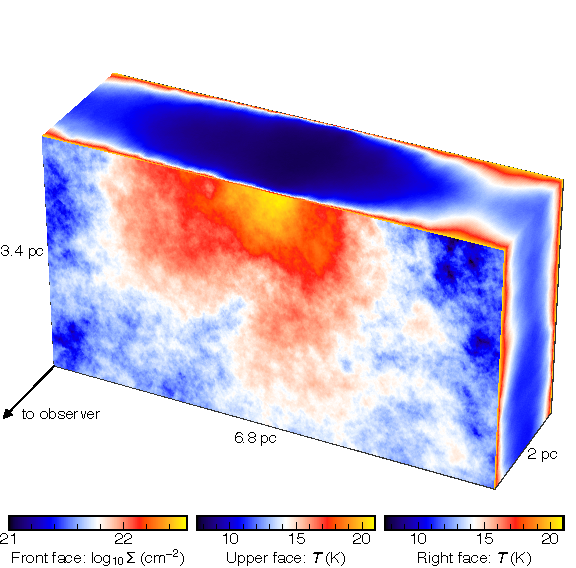
\includegraphics[width=\columnwidth]{fig_cube3d.pdf}
\caption{A cut-away view of the radiative transfer model of the cloud, seen from the observer's side. The front face is the surface 
density map of the lower half of the field, oriented as in Fig.~\ref{fig:simsky6}; the depth runs along the line of sight. The 
upper face is a cut through the middle row of the field, and the right face a cut along its last column. Both show the dust 
temperature in the plane of the cut.}
\label{fig:cube3d}
\end{figure}

\begin{figure*}
\centering
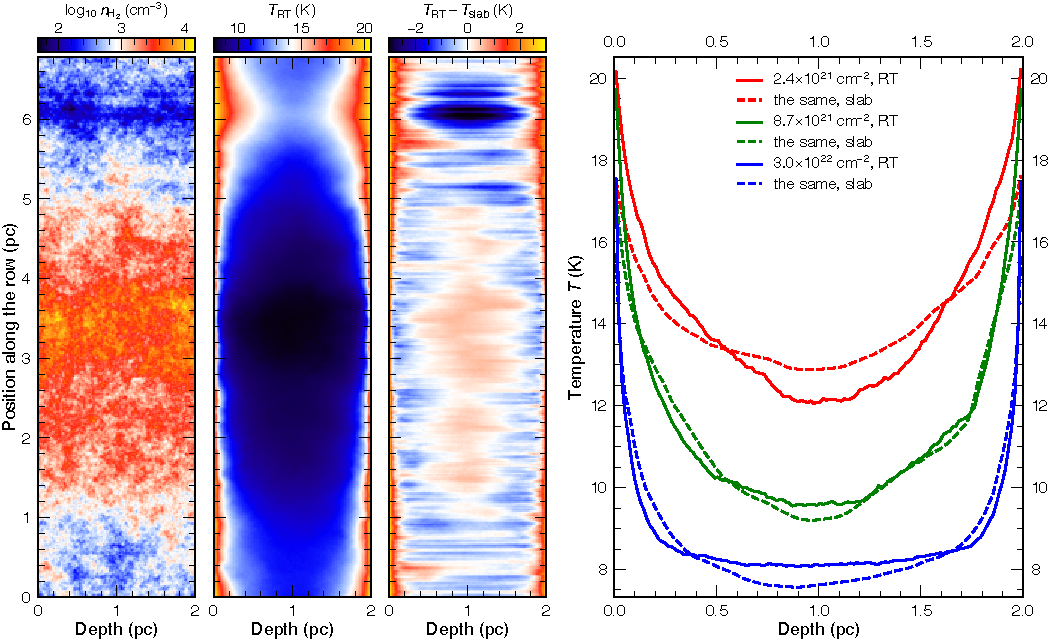
\includegraphics[width=0.9\textwidth]{fig_cube.pdf}
\caption{A slice through the radiative transfer model of the cloud, along the middle row of the field (vertical axis) and the line
of sight (horizontal axis). The depth along the line of sight is horizontal in all four panels. \emph{Left three panels}: the H$_2$
number density, the dust temperature, and the difference between the dust temperature and that of the analytic slab with the same
surface density in each column. \emph{Right panel}: the dust temperature against the depth for three columns of different surface
density, in the radiative transfer model (solid) and in the analytic slab (dashed).}
\label{fig:cube}
\end{figure*}

As a result, the emission of the radiative transfer model at 160{\um} is up to 1.5 times that of the analytic slab with the same
surface density. In the simulated sky, the emission of the analytic slab is multiplied in each band by the ratio of the emission of
the radiative transfer model to that of the slab, computed in each cell and interpolated to the pixels. The sky thus has the
temperatures of the radiative transfer model and the fine structure of the map of the cloud.

\section{The arrangement of the material along the line of sight}
\label{app:arrange}

The correction is applied pixel by pixel. A pixel receives the emission of everything along its line of sight, and a single modified
blackbody is fitted to this sum. The fit is therefore biased by the whole distribution of dust temperatures along the line of sight,
not by the temperature of any one structure. The method replaces this distribution by the one of a single uniform body with the
same total surface density. This appendix measures the error of this replacement.

In a plane-parallel geometry, the emergent emission depends only on the total surface density (Eq.~\ref{eq:invariance}).

\subsection{Concentration}
\label{app:concentr}

In the plane-parallel limit, the density profile has no effect at all. Concentration can therefore act only through the radiation
that escapes across the line of sight. A bounded structure allows this escape, and a layer does not. We measure the effect on a
sphere with the density $\rho(r) \propto (1 + r^2/a^2)^{-1}$ out to its boundary. The sphere is normalized so that the column
through its center equals the observed one, and $a$ is set by the central-to-edge density ratio. The parcels along the central line
of sight are weighted by their density, as in the emission. For each parcel, the column is integrated along the ray to the
boundary in every direction of the average.

\begin{table}
\caption{Correction factor required by the central line of sight of a sphere of the given central surface density, for four
central-to-edge density ratios. The first column is a uniform sphere.}
\label{tab:concentr}
\centering
\begin{tabular}{lcccc}
\hline\hline
\noalign{\smallskip}
$\Sigma$ (cm$^{-2}$) & uniform & $10$ & $10^2$ & $10^3$ \\
\noalign{\smallskip}
\hline
\noalign{\smallskip}
$5{\times}10^{21}$ & $1.087$ & $1.124$ & $1.155$ & $1.172$ \\
$1{\times}10^{22}$ & $1.270$ & $1.323$ & $1.392$ & $1.437$ \\
$3{\times}10^{22}$ & $1.722$ & $1.776$ & $1.906$ & $2.045$ \\
$1{\times}10^{23}$ & $1.898$ & $1.940$ & $2.043$ & $2.228$ \\
\noalign{\smallskip}
\hline
\end{tabular}
\end{table}

Table~\ref{tab:concentr} gives the result. Concentration always raises the required correction, because the mass of a concentrated
structure lies where the shielding is deepest. The effect is 2 to 4\% for a density ratio of 10 and 8 to 19\% for a ratio of $10^3$.
It is one-sided. A correction built on uniform structures therefore underestimates the deficit of a concentrated structure and never
overestimates it.

\subsection{Two superposed components}
\label{app:twocomp}

The second case is a line of sight that crosses a cloud with a denser structure embedded in it at an unknown depth. We take
a plane-parallel cloud of surface density $\Sigma_{\rm c}$. The material at the column depth $x$ in the cloud is shielded by the
angular average of $x/|\mu|$ toward the observer and of $(\Sigma_{\rm c} - x)/|\mu|$ away from the observer. A uniform sphere with the
surface density $\Sigma_{\rm s}$ through its center is embedded in the cloud. A fraction $q$ of the cloud lies in front of the
sphere. A parcel at the signed position $z$ along the diameter of the sphere, in units of its radius, is shielded by its own sphere
over the path
\begin{equation}
   l(z,\psi) = -z\cos\psi + \sqrt{1 - z^2\sin^2\psi} ,
\label{eq:lsphere}
\end{equation}
in units of the radius. It is also shielded by the cloud over $q\,\Sigma_{\rm c}/|\cos\psi|$ toward the observer and
$(1-q)\,\Sigma_{\rm c}/|\cos\psi|$ away from the observer. We take the angular average of Eq.~(\ref{eq:seff}) over $\psi$ with the
isotropic weight $\sin\psi$. The temperature of every parcel follows from Eq.~(\ref{eq:law}). The emission of the cloud and of the
sphere are added with their masses, and one modified blackbody is fitted to the sum, exactly as in the reconstruction. This gives
the fitted surface density $\Sigma_{\rm f}$ of the composite line of sight and the factor $\Sigma/\Sigma_{\rm f}$ that it requires.
The method sees only $\Sigma_{\rm f}$ and applies $f(\Sigma_{\rm f})$ of Eq.~(\ref{eq:factor}). The error of the corrected surface
density is therefore $f(\Sigma_{\rm f})\,\Sigma_{\rm f}/\Sigma - 1$.

\begin{figure*}
\centering
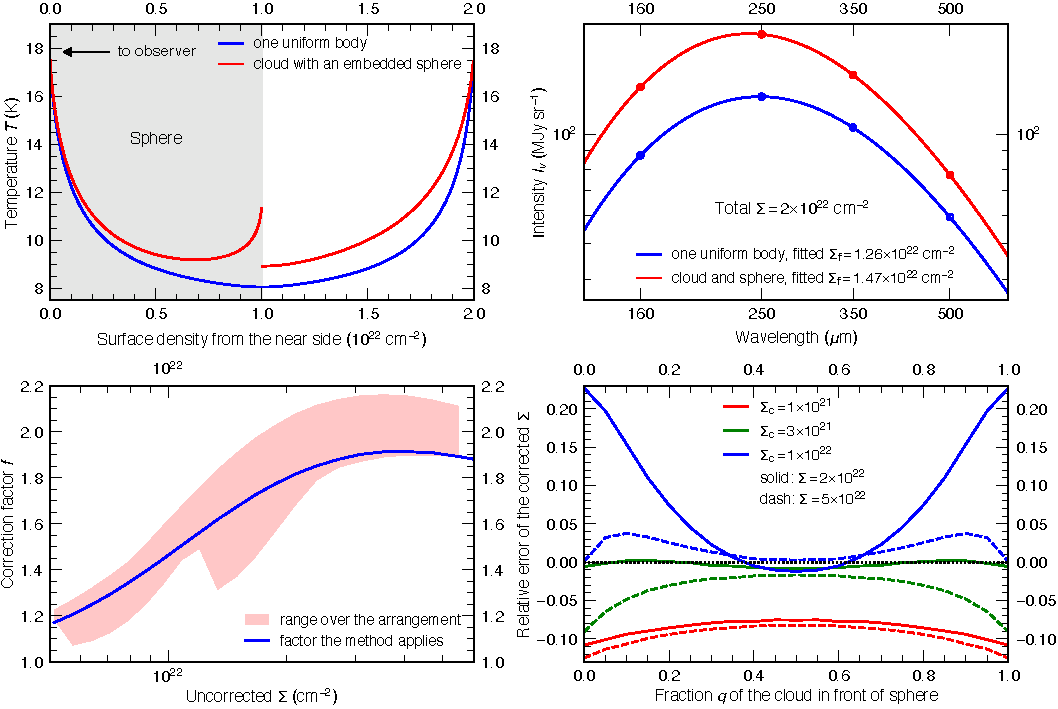
\includegraphics[width=0.98\textwidth]{fig_superposition.pdf}
\caption{Superposition of a cloud and a sphere. \emph{Upper left}: The dust temperature along a line of sight of
$2{\times}10^{22}$\,cm$^{-2}$. One curve is for the uniform body that the method assumes. The other curve is for the same surface
density divided equally between a cloud and a uniform sphere at the near side of the cloud ($q = 0$). \emph{Upper right}: The
emission of the two lines of sight, with the surface density $\Sigma_{\rm f}$ that a single modified blackbody fit returns. The two
lines of sight have the same true surface density. \emph{Lower left}: The factor that the method applies and the range of factors
that the composite lines of sight require, both against the observed (fitted) surface density. The range covers cloud surface
densities $\Sigma_{\rm c}$ of $10^{21}$, $3{\times}10^{21}$ and $10^{22}$\,cm$^{-2}$ and all positions of the sphere. \emph{Lower
right}: Relative error of the corrected surface density against the fraction $q$ of the cloud in front of the sphere. Colors give 
the surface density of the cloud $\Sigma_{\rm c}$; solid and dashed curves are for total surface densities of $2{\times}10^{22}$ and 
$5{\times}10^{22}$\,cm$^{-2}$.}
\label{fig:superposition}
\end{figure*}

Figure~\ref{fig:superposition} gives the result. The error of the corrected surface density ranges from $-13$ to $+23$\%. Its sign
depends on the cloud. A weak cloud ($\Sigma_{\rm c} = 10^{21}$\,cm$^{-2}$) leaves the sphere nearly isolated. The sphere needs more
correction than the average of a sphere and a layer, so the correction is too small by 8 to 13\%, at any depth. A dense cloud
($\Sigma_{\rm c} = 10^{22}$\,cm$^{-2}$) with the sphere at one of its sides makes the line of sight warmer than a single body. The
correction is then too large, by up to 23\%. When the sphere lies near the middle of a dense cloud, the error is only a few
percent. The simulated sky of Sect.~\ref{sec:sim}, built entirely from radiative
transfer models, shows both regimes: the wings of filaments in its weak outer cloud are corrected too little, and the flanks of
filaments in its dense central cloud too much.

The upper panels of Fig.~\ref{fig:superposition} show why the effect exists. A sphere at the near side of the cloud loses radiation
sideways, and nothing in front of it blocks the incoming radiation. This line of sight is warmer and brighter than the uniform body
of the same surface density. A single modified blackbody fit returns $1.47{\times}10^{22}$\,cm$^{-2}$ for it and
$1.26{\times}10^{22}$\,cm$^{-2}$ for the uniform body. The composite line of sight requires a factor of 1.36, but the method sees
$1.47{\times}10^{22}$\,cm$^{-2}$ and applies the factor that a uniform body with this observed surface density requires, which is
1.67. The corrected surface density is then 23\% too high.

Nothing observable distinguishes the two lines of sight, so this error is an irreducible uncertainty of any method of this kind.

\section{Why the observed colors cannot supply the correction}
\label{app:colors}
\label{sec:amplification}

One could try to measure the temperature structure directly, by fitting more than one component to the observed spectrum of each
line of sight. Without noise, this works. A free two-temperature fit from 160 to 500{\um} recovers 0.96 to 1.00 of the true surface
density at the centers of the four models, against 0.62 to 0.91 for the single-temperature fit. With noise, it does not work.
Table~\ref{tab:signature} shows why.

\begin{table}
\caption{Signature of the temperature mixing in the four-band spectral energy distribution at the center of each model, compared
with the deficit it produces. Columns two to five give the relative residuals, in percent, of the best single-component fit to the
noiseless intensities; column six their root-mean-square; column seven the fraction of the true surface density that the
single-component fit recovers.}
\label{tab:signature}
\centering
\begin{tabular}{lcccccc}
\hline\hline
\noalign{\smallskip}
$\rho_{\rm c}/\rho_{\rm e}$ &\!\!\!\! 160\,$\mu$m &\!\!\!\! 250\,$\mu$m &\!\!\!\! 350\,$\mu$m &\!\!\!\! 500\,$\mu$m &\!\!\!\! rms &\!\!\! recovery\\
\noalign{\smallskip}
\hline
\noalign{\smallskip}
1.18  &\!\!\!\! $+0.92$ &\!\!\!\! $-1.37$ &\!\!\!\! $-0.44$ &\!\!\!\! $+0.93$ &\!\!\!\! 0.97 &\!\!\!\ 0.914\\
1.28  &\!\!\!\! $+0.88$ &\!\!\!\! $-2.16$ &\!\!\!\! $-0.46$ &\!\!\!\! $+1.82$ &\!\!\!\! 1.50 &\!\!\!\ 0.869\\
4.47  &\!\!\!\! $+3.46$ &\!\!\!\! $-6.44$ &\!\!\!\! $-1.56$ &\!\!\!\! $+5.39$ &\!\!\!\! 4.61 &\!\!\!\ 0.680\\
90.8  &\!\!\!\! $+3.76$ &\!\!\!\! $-8.04$ &\!\!\!\! $-1.64$ &\!\!\!\! $+7.27$ &\!\!\!\! 5.79 &\!\!\!\ 0.619\\
\noalign{\smallskip}
\hline
\end{tabular}
\end{table}

The residuals have the same pattern for every model: positive at 160 and 500{\um} and negative at 250 and 350{\um}. This is the
broadening of the spectrum by a mixture of temperatures. The deficit divided by the root-mean-square residual is 8.9, 8.7, 6.9 and
6.6. Any method that infers the deficit from the colors therefore amplifies the relative photometric errors by a factor of 7 to 9.
The calibration uncertainties of \emph{Herschel} observations of Aquila are 20\% at 70 to 160{\um} and 10\% at 250 to 500{\um}
\citep{Konyves+2015}. For the two weakly concentrated models, the whole signature is below the photometric accuracy, and a test that accepts a second
component only where it significantly improves the fit never accepts it (Fig.~\ref{fig:mixing}). The correction must therefore be
calibrated on models in which the answer is known.

\begin{figure*}
\centering
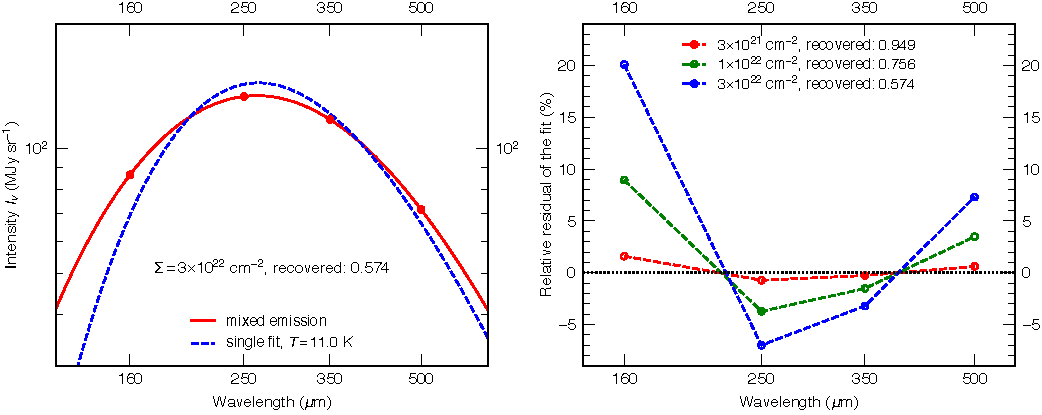
\includegraphics[width=0.98\textwidth]{fig_mixing.pdf}
\caption{\emph{Left}: the emission of a line of sight of $3{\times}10^{22}$\,cm$^{-2}$, the sum over depth of material at every
temperature, with the single modified blackbody fitted to it in the four wavebands and with the weights that the reconstruction
uses. The fit is drawn toward the warmer and brighter material, so the temperature it returns is too high and the surface density
that follows from it is too low. \emph{Right}: the relative residuals of that fit, waveband by waveband, for three total surface 
densities, with the fraction of the true surface density recovered beside each. The pattern is always the same, positive at the ends 
and negative in the middle, and it grows with the surface density, but it never rises above the calibration uncertainties of 20{\%} 
at 160{\um} and 10{\%} at the three longer wavebands.}
\label{fig:mixing}
\end{figure*}



\section{The radiation field}
\label{app:field}

The relation of Eq.~(\ref{eq:law}) was measured for a single field, $G_0 = 10$. A stronger field heats the dust at every
attenuating column, and this changes the deficit of the fit. To measure the effect, we tested the correction on the grid of
radiation fields of Appendix~\ref{sec:grid}, comparing for every pixel the factor that restores its true surface density with the
factor that the correction applies. The first column of Table~\ref{tab:fieldR} gives
the relative error of the corrected surface density without the field factor. The error changes sign twice: the correction is too
large in the weakest fields, too small in fields of a few tens, and again too large at the highest surface densities in the
strongest fields. The deficit of a single-temperature fit depends on how the temperature varies along the line of sight, and a
stronger field changes this variation differently at different depths. No simple rescaling of Eq.~(\ref{eq:law}) with the field can
therefore reproduce the errors.

\subsection{The field factor $g$}
\label{app:fieldR}

The field factor $g(\Sigma_{\rm f}, G_0)$ of Eq.~(\ref{eq:factorg0}) is measured on the same grid. For each field, the factor that each
pixel of each model requires is tabulated against the fitted surface density. Its logarithm is averaged over the pixels in bins of
0.1\,dex of $\Sigma_{\rm f}$ and smoothed over three bins. The field factor is the ratio of this average to the same average at
$G_0 = 10$. Bins with fewer than $2{\times}10^4$ pixels take the value of the nearest populated bin, and above
$10^{22.6}$\,cm$^{-2}$ the field factor is held at its value there. Table~\ref{tab:fieldR} gives the errors of the corrected surface
density, without and with the field factor, and with the field factor built without the field being tested.

\begin{table}
\caption{Relative error of the corrected surface density, in percent, for the models of the grid of radiation fields, in four ranges
of $\log_{10}\Sigma_{\rm f}$ (cm$^{-2}$): 21.6--22.0, 22.0--22.4, 22.4--22.8 and 22.8--23.4. Each entry is the median over the
pixels in the range. The rows give the correction without the field factor $g$, with $g$ built from all nine fields, and with $g$ built
without the field tested (left out). The factor is held at its maximum in all rows.}
\label{tab:fieldR}
\centering
\setlength{\tabcolsep}{4pt}
\begin{tabular}{rccc}
\hline\hline
\noalign{\smallskip}
$G_0$ & without $g$ & with $g$ & left out \\
\noalign{\smallskip}
\hline
\noalign{\smallskip}
0.98  & $+15$ $+27$ $+21$ $+16$ & $+4$ $-2$ $-5$ $-9$  & -- \\
2.12  & $+14$ $+22$ $+15$ $+10$ & $+2$ $-3$ $-4$ $-9$  & $+2$ $-1$ $-3$ $-8$ \\
4.61  & $+8$ $+11$ $+7$ $-2$    & $+3$ $-1$ $-4$ $-10$ & $+3$ $-1$ $-3$ $-11$ \\
10.0  & $+1$ $-2$ $-5$ $-13$    & $+1$ $-2$ $-5$ $-13$ & -- \\
21.7  & $-7$ $-12$ $-12$ $-19$  & $+1$ $-3$ $+3$ $-5$  & $0$ $-5$ $-4$ $-11$ \\
47.1  & $-12$ $-19$ $-19$ $-20$ & $+1$ $-4$ $-2$ $-3$  & $-1$ $-9$ $-7$ $-8$ \\
102.4 & $-12$ $-15$ $-13$ $-12$ & $+1$ $-4$ $-3$ $-2$  & $-2$ $-7$ $-5$ $-4$ \\
222.2 & $-8$ $-7$ $+1$ $+5$     & $0$ $-3$ $-1$ $+3$   & $0$ $-6$ $-2$ $+1$ \\
482.5 & $-1$ $+6$ $+17$ $+24$   & $0$ $-3$ $0$ $+6$    & -- \\
\noalign{\smallskip}
\hline
\end{tabular}
\end{table}

With the field factor, the error no longer depends on the field. In every field, it is close to the error at $G_0 = 10$, and within
$\pm 10$\% except in the densest range. The remaining deficit of up to 13\% in the densest range is the deficit at the centers of
concentrated cores. When a field is left out, its errors grow by a few percent, which measures the error of interpolating between
the fields of the grid.

\subsection{Estimating the field that a cloud requires}
\label{app:fieldest}

The field of a cloud is estimated from the temperatures that the reconstruction fits, by comparing them with those of the models at
the same surface density. For each field of the grid, the median fitted temperature of the models is tabulated in bins of 0.2\,dex of
the fitted surface density. At a fixed surface density, this temperature rises monotonically with the field. An observed temperature
is therefore converted into the field that the models need to reach it, by interpolating $\log G_0$ against the median temperature.
The procedure uses only the surface density and temperature images at the resolution of the harvested models, $13.5{\arcsec}$, and it
is carried out by the script \texttt{g0\_requirement.py}.

The simple scaling $T \propto G_0^{1/(4+\beta)}$ \citep{IvezicElitzur1997, Tielens2005}, which gives $T \propto G_0^{1/6}$ for our
dust, is not used. It holds for dust that is optically thin to the heating radiation. At a fixed surface density, the fitted
temperature of the models rises only as $G_0^{0.09}$ to $G_0^{0.13}$, because the shielded dust is heated by an attenuated and redder
field and partly by the floor component. The simple scaling would place a cloud at a field several times too weak.

The field is taken from the diffuse material only, below $10^{21.8}$\,cm$^{-2}$. In denser bins, the fields that the procedure gives
rise steadily with the surface density in every cloud. Table~\ref{tab:g0aquila} shows this for Aquila, where the median field rises
from about 20--40 in the diffuse bins to more than 100 in the densest ones. The rise is found even in Scorpius, which contains no
strong heating source. It is therefore a bias, not a real increase of the field. A dense structure seen through warm diffuse material
has a higher fitted temperature than an isolated core of the same surface density, and the procedure attributes the extra warmth to
the field. Pixels warmer than the strongest field of the grid allows are counted separately. They are heated internally, by
protostars, or by nearby massive stars beyond the range of the grid.

\begin{table}
\caption{The procedure of Appendix~\ref{app:fieldest} applied to the whole Aquila map at $13.5{\arcsec}$. Pixels: the number of
pixels in each bin of $\log_{10}\Sigma$, with $\Sigma$ in cm$^{-2}$. $T$: the fitted temperature at the 16th, 50th and 84th
percentiles of the pixels in the bin. $G_0$: the fields that reproduce these temperatures; $>$482 marks a temperature above the
strongest field of the grid. Too warm: the fraction of pixels above the strongest field.}
\label{tab:g0aquila}
\centering
\footnotesize
\setlength{\tabcolsep}{2pt}
\begin{tabular}{lrccr}
\hline\hline
\noalign{\smallskip}
$\log_{10}\Sigma$ & Pixels & $T$ (K) & $G_0$ & Too warm \\
\noalign{\smallskip}
\hline
\noalign{\smallskip}
21.0--21.2 & 370\,582 & 19.2--19.7--20.0 & 21--25--27 & 0.0{\%} \\
21.2--21.4 & 9\,527\,486 & 18.4--19.0--19.4 & 16--21--24 & 0.0{\%} \\
21.4--21.6 & 14\,764\,152 & 17.7--18.4--19.1 & 29--38--50 & 0.0{\%} \\
21.6--21.8 & 3\,573\,950 & 16.7--17.4--17.9 & 47--63--78 & 0.6{\%} \\
21.8--22.0 & 837\,305 & 15.7--16.6--18.3 & 56--87--205 & 8.2{\%} \\
22.0--22.2 & 242\,512 & 14.6--15.5--17.8 & 51--81--299 & 10.9{\%} \\
22.2--22.4 & 76\,237 & 13.8--14.5--16.5 & 62--94--284 & 10.2{\%} \\
22.4--22.6 & 23\,438 & 13.3--13.9--16.0 & 74--94--295 & 11.3{\%} \\
22.6--22.8 & 8\,368 & 12.8--13.5--15.8 & 73--118--$>$482 & 17.6{\%} \\
22.8--23.0 & 2\,874 & 12.0--13.5--15.5 & 109--252--$>$482 & 28.0{\%} \\
23.0--23.2 & 546 & 13.6--14.6--15.9 & 343--$>$482--$>$482 & 69.8{\%} \\
\noalign{\smallskip}
\hline
\end{tabular}
\end{table}

The field of a cloud is the median, weighted by the number of pixels, of the fields of its diffuse bins. The fields at the 16th and
84th percentiles of the temperature give its spread. Table~\ref{tab:g0regions} lists the result for nine regions. Their diffuse
fields span more than two orders of magnitude, from below 1 in Taurus and about 5 in California and Perseus to about 250 in
Cygnus~X. Only Scorpius and Orion~A are close to the field $G_0 = 10$ of the calibration. In Taurus, the diffuse dust (13.6 to
14.4\,K between $10^{21}$ and $10^{21.4}$\,cm$^{-2}$) is colder than the models in the weakest field of the grid (14.9\,K), and the
procedure gives only an upper limit. The correction then uses the field factor of $G_0 = 0.98$. Between $G_0 = 0.98$ and 2.12, the errors of the correction without $g$
change by only 1 to 6\% (Table~\ref{tab:fieldR}), so this approximation changes the corrected $\Sigma$ by a few percent at most. Taurus is heated by about the local interstellar field, of order
unity in Habing units, so the estimated fields are not physical field strengths. They would all change if the real dust emitted more
or less efficiently than the dust of the models. The correction is consistent nevertheless, because $g$ is measured on the same
dust. \draftnote{References for the images of all regions.}

\begin{table}
\caption{The fields of nine regions, from the diffuse material below $10^{21.8}$\,cm$^{-2}$ (Appendix~\ref{app:fieldest}). $G_0$:
the fields that reproduce the 16th, 50th and 84th percentiles of the fitted temperature, as medians over the diffuse bins weighted by
their pixels. Too warm: the fraction of all pixels of the map warmer than the strongest field of the grid allows.}
\label{tab:g0regions}
\centering
\begin{tabular}{lcr}
\hline\hline
\noalign{\smallskip}
Region & $G_0$ & Too warm \\
\noalign{\smallskip}
\hline
\noalign{\smallskip}
Taurus        & $<$0.98           & 0.0{\%} \\
California    & 3.6 -- 5.4 -- 6.9 & 0.1{\%} \\
Perseus       & 3.2 -- 4.7 -- 6.1 & 0.1{\%} \\
Scorpius      & 6.2 -- 7.9 -- 10  & 0.0{\%} \\
Orion~A       & 5.9 -- 8.9 -- 28  & 2.0{\%} \\
Ophiuchus     & 14 -- 31 -- 55    & 0.7{\%} \\
Aquila        & 25 -- 33 -- 41    & 0.4{\%} \\
W3, W4, W5    & 54 -- 62 -- 73    & 1.3{\%} \\
Cygnus~X      & 200 -- 250 -- 320 & 21.8{\%} \\
\noalign{\smallskip}
\hline
\end{tabular}
\end{table}

A single field per cloud is an approximation. In Orion~A and Ophiuchus, the fields at the 16th and 84th percentiles differ by a
factor of four or five, because parts of these clouds are lit by nearby OB stars. For such clouds, the map can be divided into
regions with their own fields. In Cygnus~X, a fifth of the pixels are warmer than the strongest field of the grid allows, and the
correction is not calibrated for them.

\section{Why the sphere and the layer are the limits}
\label{app:shape}

\begin{figure*}
\centering
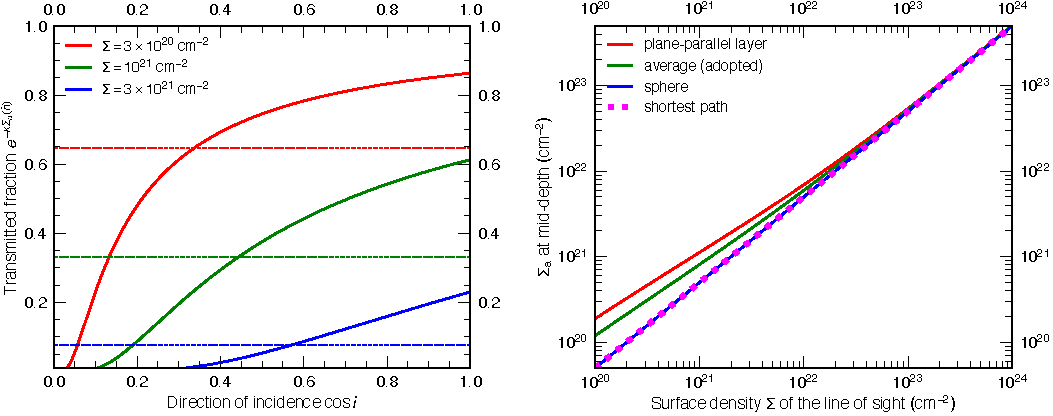
\includegraphics[width=0.98\textwidth]{fig_angular.pdf}
\caption{\emph{Left}: The fraction of the heating radiation that survives the journey inward, against the direction it comes from, 
for a parcel at mid-depth of a plane-parallel layer of three total surface densities. Plotted against the cosine of the angle, the
angular mean of each curve is the area beneath it, drawn dashed; the single column that would produce that same mean intensity is
the effective attenuating column of Eq.~(\ref{eq:seff}). \emph{Right}: that column against the total surface density of the line of
sight, for the two limiting shapes and for the average of them that is adopted, with the shortest path for comparison.}
\label{fig:angular}
\end{figure*}




The cube in Fig.~\ref{fig:relation} shows that the sphere and the layer are indeed the limits. The cube has the symmetry of neither
of them. Its factor lies between them at every surface density, within 6\% of the sphere and within 3\% of the layer. The layer is an
extreme case because it is unbounded across the line of sight. For a parcel at the mid-plane, the path to the boundary is the
half-thickness divided by the cosine of the angle to the normal. This path diverges as the angle approaches $90\degr$, so a whole
band of directions near the plane of the layer delivers no radiation, however thin the layer is. At $10^{22}$\,cm$^{-2}$, the
directions within $30\degr$ of the normal deliver 64\% of the mean intensity, and those within $45\degr$ deliver 93\%. In a
bounded body, the path is finite in every direction, and no direction is lost. The sphere is the opposite extreme: a compact body
with a given central surface density blocks less of the sky than any other body with that surface density. Every real cloud lies
between the two limits, and the range between them is the full effect of the shape. This is why the method needs no assumption
about the shape of a cloud.

The dotted curve of Fig.~\ref{fig:relation} shows what happens if the angular average is replaced by the column along the shortest
path, which is one quarter of the surface density when averaged over the depth of a layer. Below $3{\times}10^{21}$\,cm$^{-2}$, this simpler treatment agrees with the full calculation to 1\%.
Above $10^{22}$\,cm$^{-2}$ it diverges, and at $10^{23}$\,cm$^{-2}$ it overestimates the correction by half. The shortest path gives
too little shielding to the material near the surfaces: its column falls to zero at the surface, while the oblique directions still
shield the surface material. The surface material is then too warm, and the deficit is overestimated.

\section{Corrections that read the fitted temperature}
\label{app:tcorr}

The reconstruction gives a dust temperature for every pixel, together with the surface density. If the temperature of a pixel
differs from the one that the relation predicts at its surface density, the temperature carries information that the surface
density does not. We tested four ways of using it, all calibrated on the radiative transfer models. None was adopted, and the reason
is the same for all four.

The methods were: a table of the required factor against the surface density, the fitted temperature, and the contrast between
the images at $13.5{\arcsec}$ and $36.3{\arcsec}$; a smooth function of the surface density and of the offset of the fitted temperature
from the relation, fitted to the grid of radiation fields; a table computed from analytic lines of sight through structures embedded
in a diffuse medium; and a redistribution of the correction within each beam to follow the shape of the finest image. On the
models of the subdivision grid, they changed the median core mass by 2 to 9\% relative to the adopted correction. The third method
under-corrected the dense material in fields of $G_0 = 20$ to 50 by a factor of 1.5 to 1.7. On an earlier simulated sky, the first two
over-corrected the flanks of filaments even more than the adopted correction, and the fourth copied the noise of the finest image
into the factor.

The reason is that a warm pixel is ambiguous. A pixel can be warmer than the relation predicts for two reasons. First, a stronger
radiation field may heat it. The radiative transfer models then say that it needs more correction. Second, it may lie on the flank of
a structure, near its surface, or its line of sight may also cross a warm cloud. It then needs less correction. The models used for
the calibration contain only the first case, and the simulated sky mostly the second. A correction that uses the temperature is
therefore right in one case and wrong in the other. The fitted temperature of a single pixel cannot distinguish the two cases. The
radiation field varies over parsecs, and the warmth of a flank varies over the width of a filament. The field is therefore
estimated from the temperature of the diffuse material of the whole map, as one number for a cloud
(Appendix~\ref{app:fieldest}). In a small field, such as our Aquila cutout, only 12\% of the pixels are diffuse enough, and most of
them lie in one corner, so the field must be taken from the larger map. None of these corrections changed the core mass by more than the error due to the background (Appendix~\ref{sec:bgerr}),
so we adopted the simplest one.

\end{document}
